% CVPR 2026 Paper Template; see https://github.com/cvpr-org/author-kit

\documentclass[10pt,twocolumn,letterpaper]{article}

%%%%%%%%% PAPER TYPE  - PLEASE UPDATE FOR FINAL VERSION
% \usepackage{cvpr}              % To produce the CAMERA-READY version
% \usepackage[review]{cvpr}      % To produce the REVIEW version
\usepackage[pagenumbers]{cvpr} % To force page numbers, e.g. for an arXiv version

% Import additional packages in the preamble file, before hyperref
\usepackage{xcolor}
\usepackage{multirow}
\usepackage[T1]{fontenc}
\usepackage[utf8]{inputenc}
%% This file contains a number of tweaks that are typically applied to the main document.
%% They are not enabled by default, but can be enabled by uncommenting the relevant lines.

%%
%% Inline annotations; for predefined colors, refer to "dvipsnames" in the xcolor package:
%% https://tinyurl.com/overleaf-colors
%%
\newcommand{\red}[1]{{\color{red}#1}}
\newcommand{\todo}[1]{{\color{red}#1}}
\newcommand{\TODO}[1]{\textbf{\color{red}[TODO: #1]}}
%%
%% disable for camera ready / submission by uncommenting these lines  
%%
% \renewcommand{\TODO}[1]{}
% \renewcommand{\todo}[1]{#1}

%%
%% work harder in optimizing text layout. Typically shrinks text by 1/6 of page, enable
%% it at the very end of the writing process, when you are just above the page limit
%%
% \usepackage{microtype}

%%
%% fine-tune paragraph spacing
%%
% \renewcommand{\paragraph}[1]{\vspace{.5em}\noindent\textbf{#1.}}

%%
%% globally adjusts space between figure and caption
%%
% \setlength{\abovecaptionskip}{.5em}


%%
%% Allows "the use of \paper to refer to the project name"
%% with automatic management of space at the end of the word
%%
% \usepackage{xspace}
% \newcommand{\paper}{ProjectName\xspace}

%%
%% Commonly used math definitions
%%
% \DeclareMathOperator*{\argmin}{arg\,min}
% \DeclareMathOperator*{\argmax}{arg\,max}

%%
%% Tigthen underline
%%
% \usepackage{soul}
% \setuldepth{foobar}

% It is strongly recommended to use hyperref, especially for the review version.
% hyperref with option pagebackref eases the reviewers' job.
% Please disable hyperref *only* if you encounter grave issues, 
% e.g. with the file validation for the camera-ready version.
%
% If you comment hyperref and then uncomment it, you should delete *.aux before re-running LaTeX.
% (Or just hit 'q' on the first LaTeX run, let it finish, and you should be clear).
\definecolor{cvprblue}{rgb}{0.21,0.49,0.74}
\usepackage[pagebackref,breaklinks,colorlinks,allcolors=cvprblue]{hyperref}

%%%%%%%%% PAPER ID  - PLEASE UPDATE
\def\paperID{*****} % *** Enter the Paper ID here
\def\confName{CVPR}
\def\confYear{2026}

%%%%%%%%% TITLE - PLEASE UPDATE
\title{{\ourmethod}: Instant 3D Scene Editing from Sparse Unposed Images}

% For a paper whose authors are all at the same institution,
% omit the following lines up until the closing ``}''.
% Additional authors and addresses can be added with ``\and'',
% just like the second author.
% To save space, use either the email address or home page, not both
%%%%%%%%% AUTHORS - PLEASE UPDATE

\author{
Jiageng Liu$^{*}$\\
University of Massachusetts Amherst\\
{\tt\small jiagengliu@umass.edu}
\and
Weijie Lyu$^{*}$\\
University of California, Merced \\
{\tt\small wlyu3@ucmerced.edu}
\and
Xueting Li\\
NVIDIA\\
{\tt\small xuetingl@nvidia.com}
\and
Yejie Guo\\
Shanghai Jiao Tong University\\
{\tt\small gyj123@sjtu.edu.cn}
\and
Ming-Hsuan Yang\\
University of California, Merced \\
{\tt\small myang37@ucmerced.edu}
}
\newcommand{\ourmethod}{\textit{Edit3r}}
\newcommand{\ourbench}{\textit{DL3DV-Edit-Bench}}
\newcommand{\XT}[1]{{\color{orange}[XT: #1]}}

\begin{document}

\twocolumn[{% 
\renewcommand\twocolumn[1][]{#1}% 
\maketitle
\begin{center}
% \vspace{-0.2in}
\vspace{-8mm}
\centering 
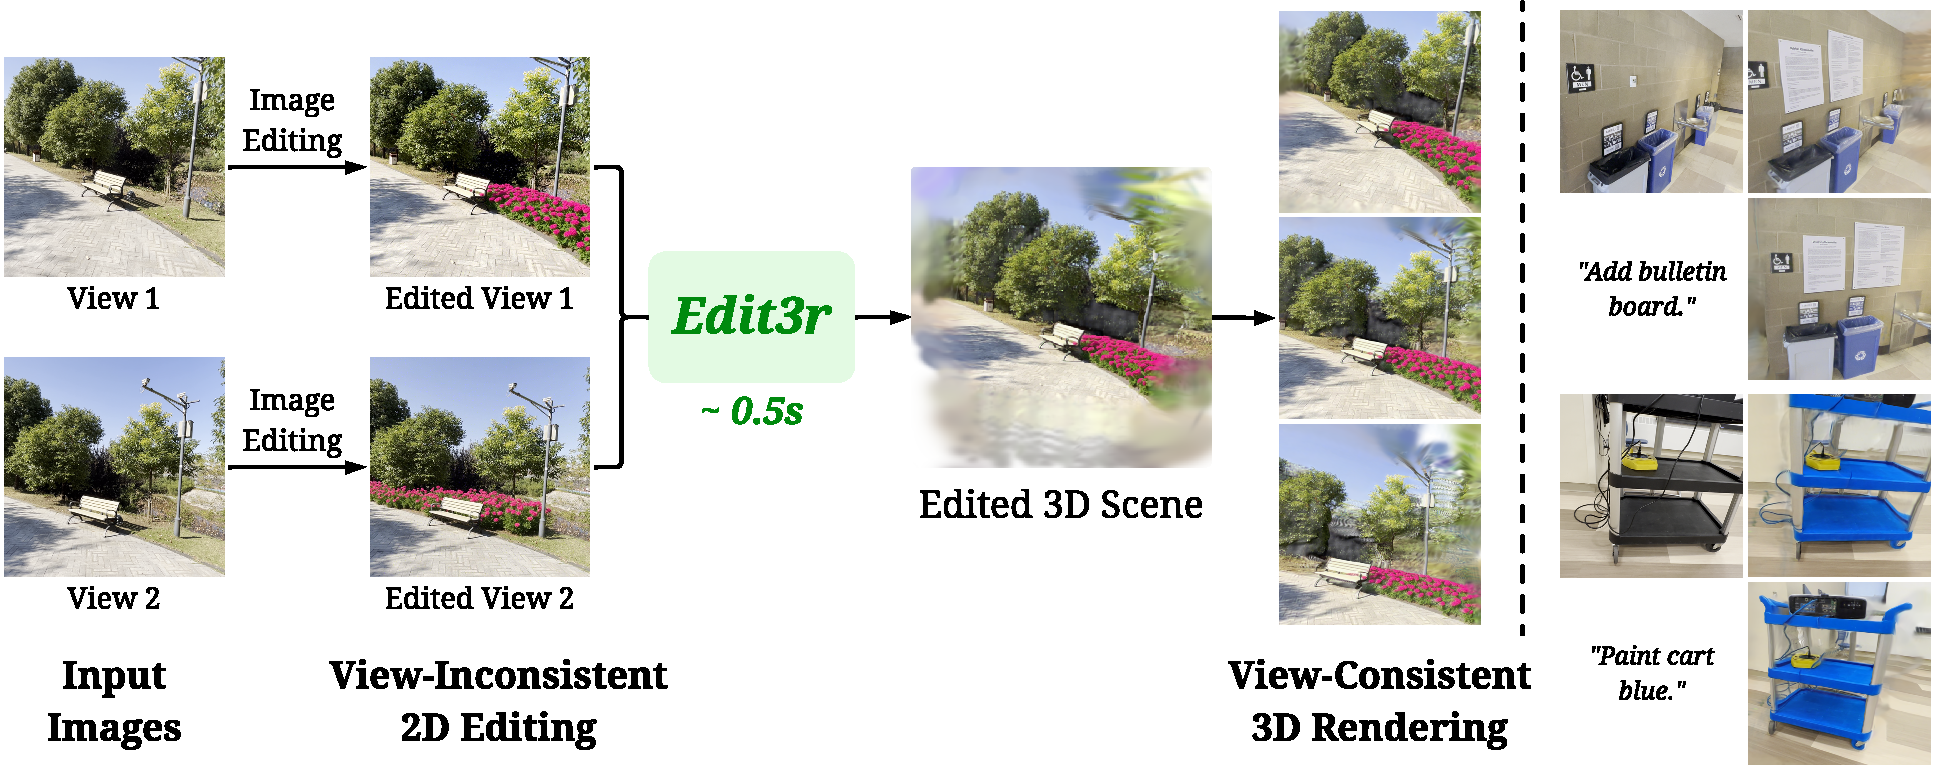
\includegraphics[width=0.95\linewidth]{fig/teaser_v5.pdf}
    \captionsetup{width=\linewidth}
    \captionof{figure}{\textbf{Overview.} {\ourmethod} takes view-inconsistent, 2D edited images as input and generates a view-consistent 3D scene for novel view synthesis in only 0.5 seconds. It supports diverse editing tasks, including insertion, removal, color changes, and weather changes, \etc.}
    \label{fig:teaser}
    \vspace{4mm}
\end{center}
}]
\begingroup
\renewcommand{\thefootnote}{\fnsymbol{footnote}}
\footnotetext[1]{These authors contributed equally.}
\endgroup

\begin{abstract}
%
We present \textbf{\ourmethod}, a feed-forward framework that reconstructs and edits 3D scenes in a single pass from unposed, view-inconsistent, instruction-edited images.
%
Unlike prior methods requiring per-scene optimization, {\ourmethod} directly predicts instruction-aligned 3D edits, enabling fast and photorealistic rendering without optimization or pose estimation.
%
A key challenge in training such a model lies in the absence of multi-view consistent edited images for supervision. We address this with (i) a SAM2-based recoloring strategy that generates reliable, cross-view-consistent supervision, and (ii) an asymmetric input strategy that pairs a recolored reference view with raw auxiliary views, encouraging the network to fuse and align disparate observations.
%
At inference, our model effectively handles images edited by 2D methods such as InstructPix2Pix, despite not being exposed to such edits during training.
%
For large-scale quantitative evaluation, we introduce \textbf{{\ourbench}}, a benchmark built on the DL3DV test split, featuring 20 diverse scenes, 4 edit types and 100 edits in total.
%
Comprehensive quantitative and qualitative results show that {\ourmethod} achieves superior semantic alignment and enhanced 3D consistency compared to recent baselines, while operating at significantly higher inference speed, making it promising for real-time 3D editing applications.
\textbf{Project page:} \url{https://edit3r.github.io/edit3r/}.
\end{abstract}


% Scene editing受欢迎
% 但现在方法太笨
% LRM解决了这一点
% 所以我们提出了我们的方法
% 为了解决xx问题，我们主要
% （1）（2）（3）
% 实验证明我们方法有效
% 我们后续也进行了一些消融实验
% 总结
% Editing real scenes in 3D rises popularity but remains challenging, most reconstruct–edit–refit methods are optimization-based, slow and often break multi-view consistency. 
% We introduce \textbf{{\ourmethod}}, a feed-forward approach that reconstructs and edits 3D scenes in a single pass from unposed, instruction-edited views. 
% Instead of retraining per scene, {\ourmethod} directly predicts instruction-aligned 3D Gaussian splats, enabling fast, photorealistic rendering without test-time optimization or pose estimation. 
% However, Training without multi-view–consistent edited supervision is nontrivial; 
% we address this with (i) a SAM2-based recoloring strategy that yields reliable, cross-view–consistent supervision, and (ii) an asymmetric input scheme that pairs an edited reference view with unedited auxiliary views, encouraging the network to fuse and align inconsistent observations. 
% To enable fair, reproducible evaluation, we further construct \textbf{{\ourbench}} on the DL3DV test split: 20 diverse scenes with 4 edit types (Add/Remove/Modify/Global) and 100 edits total.
% With InstructPix2Pix as the default 2D editing front-end (others in ablations), {\ourmethod} achieves higher semantic alignment and stronger 3D consistency than recent baselines, while delivering substantially faster inference. 
% Quantitative results and comprehensive qualitative comparisons confirm the benefits of our training design; ablations isolate the contributions of SAM2 recoloring, asymmetric inputs, and the choice of 2D editor. 
% Together, these findings highlight {\ourmethod} as a practical solution for rapid, instruction-driven 3D scene editing.
% \end{abstract}
% \XT{    
\vspace{-2mm}
\section{Introduction}
\label{sec:intro}
3D scene editing is a long-standing problem in computer vision. By offering intuitive control over content creation, it plays a crucial role in diverse applications such as visual effects~\cite{zhang2025advancing3dgaussiansplatting}, augmented and virtual reality (AR/VR)~\cite{madhavaram2024trainingfreeapproach3d}, game design~\cite{xu2024sketch2sceneautomaticgenerationinteractive}, and digital twins~\cite{melnik2025digitaltwingenerationvisual}.
%
Recent advancements in 3D scene representation and reconstruction~\cite{nerf, 3dgs} have sparked a surge of interest in editing 3D scenes using text prompts. Existing methods~\cite{in2n, gaussctrl, lee2025editsplatmultiviewfusionattentionguided} typically combine neural reconstruction with text-driven image editing in a \textit{reconstruct-edit-refit} pipeline. Given a collection of posed images and a textual instruction, these approaches first \textit{reconstruct} the scene using a neural 3D representation, then apply 2D generative \textit{editing} to the rendered images, and finally \textit{refit} (or re-optimize) the 3D representation to incorporate the edits.
%
While this pipeline achieves impressive visual quality and alignment with instruction prompts, it is limited by slow per-scene optimization and retraining, which limits practical usability. Moreover, these methods often introduce multi-view inconsistencies, revealing a substantial gap between current 3D editing frameworks and the need for fast, interactive scene manipulation in real-world applications.

Conversely, the rapid development of Large Reconstruction Models (LRMs)~\cite{lrm, gslrm, noposplat, mvsnerf, pixelsplat, dust3r} offers a more efficient paradigm for 3D scene reconstruction by amortizing computation across large datasets and removing per-scene optimization. Notably, Gaussian-based LRMs enable rapid, photorealistic rendering suited for real-time applications, thanks to the Gaussian splatting technique.

Motivated by these advancements, we propose {\ourmethod}, a feed-forward approach that reconstructs and edits a 3D scene in a single pass.
%
Beginning with a pair of unposed views, we edit them using a 2D image editor. These potentially inconsistent edited views serve as inputs for {\ourmethod}, which directly predicts 3D Gaussian splats aligned with the edited views while eliminates the inconsistency, seamlessly unifying reconstruction and editing without the need for per-scene optimization.
% Our method takes as input a few unposed images of a scene, where a reference view is edited according to the textual instruction. From these potentially inconsistent views, \ourmethod directly predicts the 3D Gaussian splats representing the edited scene

Training such a feed-forward reconstruction-editing model introduces two practical challenges. First, ground-truth edited images for supervision are unavailable. To address this, we leverage SAM2-based recoloring~\cite{ravi2024sam} for cross-view-consistent supervision, providing reliable labels and masks. We find that our model, though trained only on a recoloring task, it effectively handles images edited by 2D diffusion models at inference. Second, edited inputs can remain semantically and visually inconsistent across views. To tackle this, we design an asymmetric input scheme that pairs recolored reference views with other views in their original appearance, encouraging the network to fuse and align edited and unedited observations.

Moreover, the lack of established benchmarks limits fair and scalable evaluation in 3D scene editing. We introduce {\ourbench}, a standardized benchmark built on the DL3DV~\cite{ling2023dl3dv10klargescalescenedataset} test split to systematically assess multi-view consistency and inference efficiency, setting a foundation for reproducible and rigorous comparisons.
%
Our contributions are summarized as follows:
\begin{itemize}
\item We introduce {\ourmethod}, a feed-forward framework that simultaneously reconstructs 3D scenes and generates edited Gaussian splats aligned to a text prompt.
\item We develop a SAM2-based recoloring technique for view-consistent supervision during training and introduce an asymmetric input scheme to bolster robustness against cross-view inconsistencies.
\item We present {\ourbench}, a scene-level, multi-view 3D editing benchmark built on the DL3DV test split.
\item Extensive quantitative and qualitative experiments show {\ourmethod} is significantly faster than previous approaches, achieving higher visual quality and semantic consistency while demonstrating practical real-world potential.
\end{itemize}




% %-------------------------------------------------------------------------
% %
% Scene editing is a long-standing problem in computer vision, enabling intuitive control over content creation across VFX, AR/VR authoring, game design, and digital-twin applications~\cite{}.
% %
% Recent advancements in 3D reconstruction techniques (\eg, Neural Radiance Fields (NeRFs) and 3D Gaussian Splatting), together with generative models that make instruction-guided editing practical from simple text prompts~\cite{}, is driving increased interest in 3D scene editing .
% %
% Several research efforts~\cite{in2n, gaussctrl} propose methods that combine neural reconstruction with text-driven image editing to enable 3D scene editing.
% Given a collection of posed images and a textual editing instruction, these approaches first reconstruct the original scene with a neural 3D representation, then apply 2D generative editing to the rendered images, and finally re-optimize or retrain the 3D representation to incorporate the edits. 
% %
% Although they deliver high visual quality and renderings aligned with the input prompts, this reconstruct–edit–refit pipeline faces practical limitations. In particular, slow optimization and retraining hinder usability, and multi-view consistency often remains fragile, leaving a gap between current 3D editing capabilities and real-world needs for rapid, interactive scene manipulation.

% % LRM介绍
% The advent of Large Reconstruction Models (LRMs)~\cite{lrm, gslrm, noposplat, mvsnerf, pixelsplat, dust3r} provides a significantly more efficient route to 3D scene reconstruction by amortizing computation across large datasets and eliminating expensive per-scene optimization.
% %
% Among them, Gaussian-based LRMs directly predicts Gaussian primitives, positions, covariances, colors, and opacities, from sparse posed views, enabling rapid, photorealistic rendering that suits real-time and practical applications.
% %
% However, current LRMs primarily aim for faithful reconstruction of static scenes rather than flexiblemanipulation or editing.
% %
% Applying LRMs on scene editing is nontrivial, as training LRMs requires multi-view consistent supervision (e.g., edited ground truth), which is rarely available; producing perfectly matched edits across views is impractical, leaving the acquisition of reliable labels as a persistent bottleneck.

% In this paper, we propose {\ourmethod}, a feed-forward approach that reconstructs and edits a 3D scene in a single pass under textual instructions.
% %
% Given a pair of unposed, sparse, instruction-edited views with remaining cross-view inconsistencies, {\ourmethod} directly predicts instruction-aligned 3D Gaussian splats in a single pass, eliminating per-scene optimization and the separation between reconstruction and editing.

% Training and evaluating such a feed-forward reconstruction–editing model raises three practical challenges. (1) Ground-truth edited images for non-reference views are unavailable, and cross-view inconsistencies persist regardless of the chosen 2D editor; we therefore derive cross-view–consistent supervision via SAM2~\cite{}-based recoloring, which provides reliable labels/masks. (2) During inference, the edited inputs remain semantically and visually inconsistent across views. To mitigate this, we adopt an asymmetric input scheme during training to manually create inconsistency: the recolored reference view is paired with other views kept in their original appearance, encouraging the network to learn to fuse and align edited and unedited observations. (3) Fair evaluation is hindered by small, ad-hoc benchmarks. We thus automate a standardized benchmark on DL3DV~\cite{}, termed {\ourbench}, to systematically assess multi-view consistency and inference efficiency, enabling reproducible comparisons.

% Our contributions are summarized as follows:
% \begin{itemize}
%     \item We propose {\ourmethod}, a feed-forward method that reconstructs the 3D scene and generates edited Gaussian splats based on the input instruction.
%     \item We propose a SAM2-recolor-based and asymmetric input training strategy to obtain view-consistent supervision during training.
%     \item We introduce {\ourbench}, a scene-level, multi-view 3D editing benchmark built on the DL3DV test split for scene editing.
%     \item Results show that our method accomplish much faster than existing apporachs with better visual quality and semantic consistency, highlighting its potential for real-world application.
% \end{itemize}

% \XT{
\section{Related Work}
\label{sec:related_work}
% \subsection{Video Segmentation and 2D Editing}

% Video editing often relies on accurate object delineation and temporally consistent propagation. Classical video object segmentation (VOS) approaches propagate masks frame-by-frame using memory networks or tracking-based heads, enabling fine-grained, object-level edits and cut-and-paste workflows. Notable lines include semi-supervised VOS with space-time memory (STM)~\cite{oh2019videoobjectsegmentationusing}, long-range memory with efficient retrieval (XMem)~\cite{cheng2022xmemlongtermvideoobject}, and tracking-by-segmentation frameworks such as MaskTrack R-CNN~\cite{yang2019videoinstancesegmentation}. Complementary tools like video inpainting~\cite{li2022endtoendframeworkflowguidedvideo} and matting allow replacing or removing objects while maintaining background coherence. Although these methods deliver strong temporal consistency, they operate purely in 2D image space and do not enforce multi-view or 3D geometric consistency.


% Recent diffusion-based 2D image editors produce high-quality, instruction- or prompt-conditioned edits. Techniques include noise-to-image guidance and partial denoising (SDEdit)~\cite{meng2022sdeditguidedimagesynthesis}, cross-attention manipulation (Prompt-to-Prompt)~\cite{hertz2022prompttopromptimageeditingcross}, instruction tuning for localized edits (InstructPix2Pix)~\cite{ip2p}, and structure-conditional control (ControlNet)~\cite{controlnet}. These methods excel at preserving layout while modifying appearance or style, but naively applying them per frame (or per view) leads to flicker and identity drift without additional temporal or geometric constraints.

% To address temporal coherence, video extensions of diffusion models reuse or constrain cross-frame features. Representative methods include one-shot or few-shot tuning for videos (Tune-A-Video)~\cite{wu2023tuneavideooneshottuningimage}, zero-shot attention reuse (Text2Video-Zero)~\cite{khachatryan2023text2videozerotexttoimagediffusionmodels}, attention/token propagation (TokenFlow)~\cite{geyer2023tokenflowconsistentdiffusionfeatures}, edit-specific attention alignment (FateZero, Video-P2P)~\cite{qi2023fatezerofusingattentionszeroshot,liu2023videop2pvideoeditingcrossattention}, and layered/implicit canonicalization (CoDeF)~\cite{ouyang2024codefcontentdeformationfields}. Systems such as Rerender~\cite{yang2023rerendervideozeroshottextguided}, AnimateDiff~\cite{guo2024animatediffanimatepersonalizedtexttoimage}, and stable video diffusion models~\cite{blattmann2023stablevideodiffusionscaling} further strengthen temporal consistency via optical-flow guidance, cross-frame attention, or structural conditioning (depth/edges). Despite impressive short-range coherence, these approaches remain fundamentally 2D: they lack explicit 3D scene reasoning, so edits do not necessarily correspond to a single, consistent 3D configuration across viewpoints. When such 2D/video edits are lifted to supervision for 3D reconstruction, view-inconsistent artifacts or geometry drift can arise. This gap motivates 3D-aware editing frameworks that couple object semantics with geometry, ensuring both temporal and multi-view consistency.

% \subsection{3D Scene Understanding and Editing}
% Recent advancements in 3D neural reconstruction methods, notably Neural Radiance Fields (NeRFs) and 3D Gaussian Splatting (3DGS), have enabled photorealistic rendering from posed images. Building upon these techniques, researchers have sought to integrate semantic information to enhance the understanding and manipulation of reconstructed 3D scenes.
% %
% Many existing works leverage semantic features~\cite{feature3dgs} or 3D segmentation~\cite{gg, gaga} to achieve 3D scene editing of specified objects. NeRF-Art~\cite{nerfart} employs global-local contrastive learning, directional constraints in the CLIP embedding space, and weight regularization to ensure that NeRF preserves its original structure during text-guided stylization. Instruct-NeRF2NeRF~\cite{ip2p} reconstructs a 3D scene with NeRF~\cite{nerf} and then edits multi-view renderings with a 2D image editing method Instruct-Pix2Pix~\cite{ip2p}, in which a text-conditioned diffusion model is trained to edit the input image that aligns coherently with the input instruction prompt. The edited images are further utilized to continue optimizing the scene. GaussianCtrl~\cite{gaussctrl} employs ControlNet~\cite{controlnet} for image editing and achieves view consistency by depth-conditioned editing to enforce geometric consistency and attention-based latent code alignment to achieve appearance consistency. GaussianEditor~\cite{gaussianeditor} enhances precision and control in editing through a proposed Gaussian semantic tracing, which traces the editing target throughout the training process.

%To eliminate per-scene optimization, DN2N~\cite{} and Free-Editor~\cite{} utilize generalizable NeRF, however, 

% \subsection{Generalizable Feed-forward Reconstructors}

% Recent advancements in large 3D reconstruction models (LRMs)~\cite{mvsnerf, murf, pixelsplat, mvsplat, noposplat, gslrm, lgm, lsm, splatter_image, facelift} have significantly accelerated 3D reconstruction tasks. Leveraging scalable transformer architectures~\cite{transformer, vit} and extensive datasets like Objaverse~\cite{objaverse, objaversexl}, these models effectively learn generalizable 3D priors. In contrast to traditional per-scene optimization methods~\cite{nerf, gs, neus}, LRMs employ a feed-forward approach, enabling rapid inference of high-quality NeRF, mesh, or 3D Gaussian representations from sparse input images in less than a second. Specific approaches such as PixelSplat~\cite{pixelsplat} utilize epipolar geometry for depth estimation, whereas methods like MVSNeRF~\cite{mvsnerf}, MuRF~\cite{murf}, and MVSplat~\cite{mvsplat} construct cost volumes for aggregating multi-view information. MVSplat360~\cite{mvsplat360} extends MVSplat by enabling 360-degree feed-forward reconstruction refined through stable video diffusion models. Similarly, DepthSplat~\cite{depthsplat} incorporates explicit depth information to enhance novel-view synthesis. Approaches such as NoPoSplat~\cite{noposplat} leverage the pose estimation capabilities of MASt3R~\cite{dust3r, mast3r} to reconstruct scenes from unposed images, while LSM~\cite{lsm} integrates reconstruction with semantic scene understanding. Despite these advancements, the application of feed-forward reconstructors in 3D scene editing and manipulation remains relatively unexplored.
\subsection{2D Image and Video Editing}
Recent diffusion-based editors enable high-quality, instruction-conditioned edits through techniques such as noise-to-image guidance~\cite{meng2022sdeditguidedimagesynthesis}, cross-attention manipulation~\cite{hertz2022prompttopromptimageeditingcross}, instruction tuning~\cite{ip2p}, and structure-conditional control~\cite{controlnet}. While effective for single images, naively applying them per frame leads to flicker and identity drift.

To address temporal coherence, video extensions employ attention/token propagation~\cite{geyer2023tokenflowconsistentdiffusionfeatures}, edit-specific attention alignment~\cite{qi2023fatezerofusingattentionszeroshot,liu2023videop2pvideoeditingcrossattention}, optical-flow guidance~\cite{yang2023rerendervideozeroshottextguided}, and implicit canonicalization~\cite{ouyang2024codefcontentdeformationfields}. Despite strong short-range coherence, these approaches remain fundamentally 2D and lack explicit 3D scene reasoning, leading to view-inconsistent artifacts when lifted to 3D supervision.

\subsection{3D Scene Editing}
Neural reconstruction methods such as NeRF~\cite{nerf} and 3D Gaussian Splatting~\cite{3dgs} enable photorealistic rendering, motivating integration with semantic editing. Existing approaches typically follow a reconstruct-edit-refit pipeline. Instruct-NeRF2NeRF~\cite{in2n} reconstructs scenes with NeRF, edits multi-view renderings using InstructPix2Pix~\cite{ip2p}, and re-optimizes the scene with edited images. GaussianCtrl~\cite{gaussctrl} employs ControlNet~\cite{controlnet} with depth conditioning and attention-based alignment for view consistency, while GaussianEditor~\cite{gaussianeditor} introduces Gaussian semantic tracing for precise editing control. Though achieving impressive quality, these methods require slow per-scene optimization and are prone to multi-view inconsistencies.

\subsection{Generalizable Feed-forward Reconstructors}
Large reconstruction models (LRMs)~\cite{mvsnerf, pixelsplat, mvsplat, noposplat, gslrm, lgm, splatter_image, lsm} have revolutionized 3D reconstruction by learning generalizable priors from large-scale datasets like Objaverse~\cite{objaverse}. Leveraging transformer architectures~\cite{transformer, vit}, these models enable rapid inference of NeRF or Gaussian representations from sparse views without per-scene optimization. Methods such as PixelSplat~\cite{pixelsplat} utilize epipolar geometry, while many other methods~\cite{mvsnerf, murf, mvsplat, mvsplat360} construct cost volumes for multi-view aggregation. Despite their efficiency in reconstruction, the application of feed-forward reconstructors to 3D scene editing remains largely unexplored, which our work addresses.
\begin{figure*}[t]  % [t]顶端；若想底部可用 [b] 并配合上面的包
    \centering
    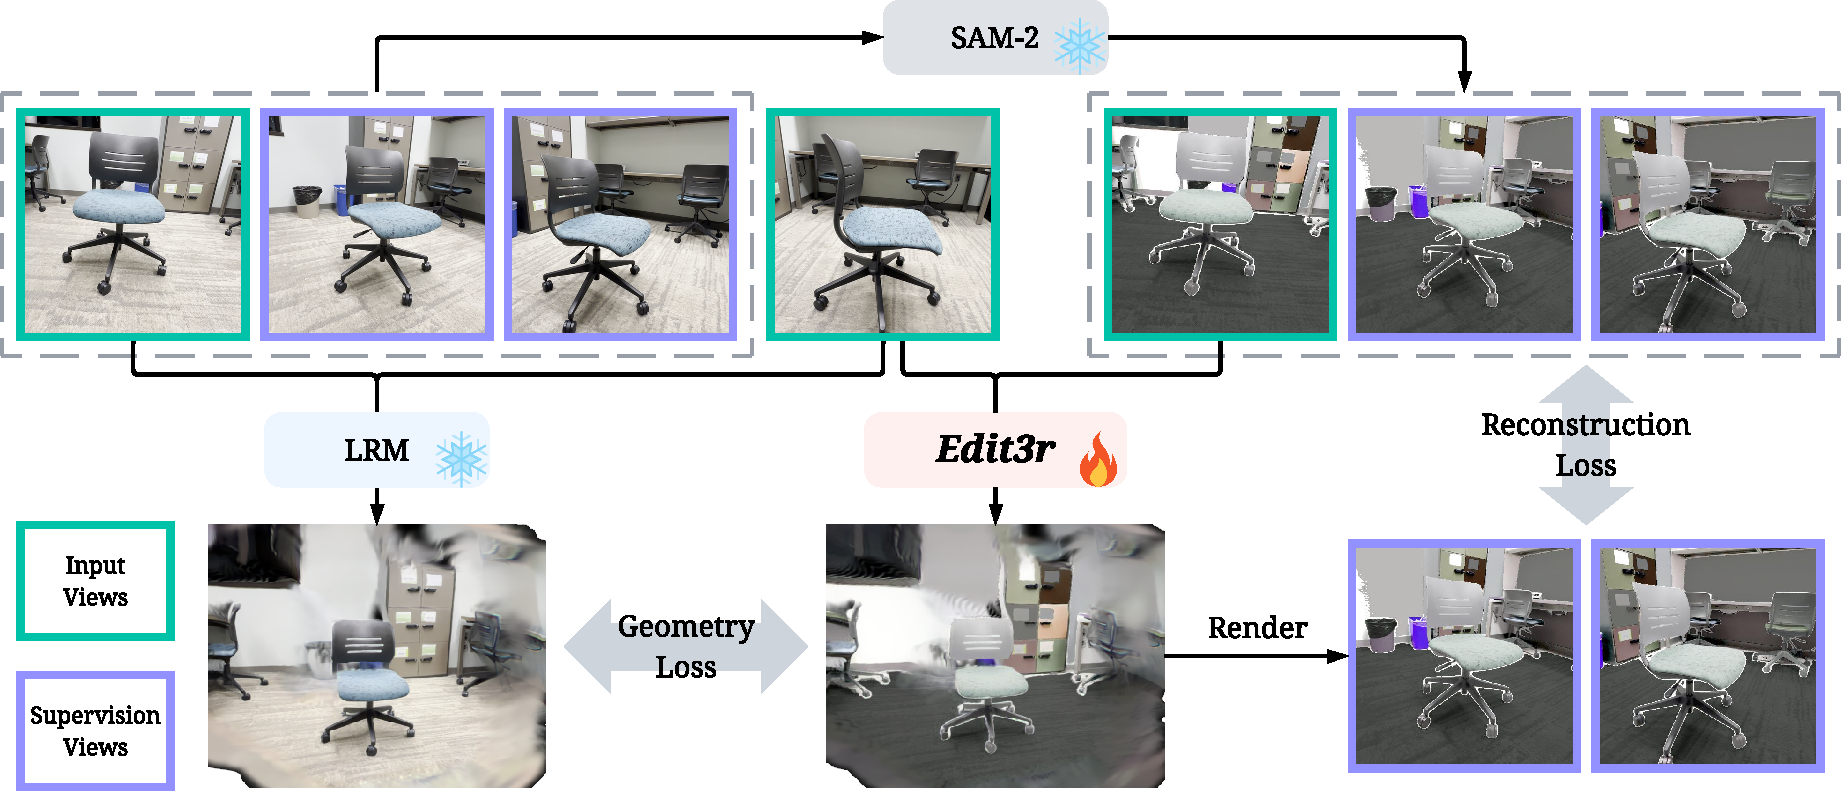
\includegraphics[width=\textwidth]{fig/pipeline_v4.pdf}
    \caption{\textbf{Training pipeline of \ourmethod.}
    Green-framed images are input views and purple-framed images are supervision views (ground-truth and rendered results).
    We first apply SAM2-based recoloring to both inputs and supervision views, then feed an asymmetric pair (one recolored view and one original view) into {\ourmethod} to predict a 3D Gaussian scene, which is rendered and supervised with reconstruction losses against the recolored supervision views (right).
    In parallel, a frozen LRM reconstructs the scene from the original inputs and provides 3D supervision via geometry losses that regularize {\ourmethod}’s Gaussian predictions in 3D space.}%绿色图片代表输入，紫色图片代表render结果和gt，我们会把输入和gt先用SAM2-based recoloring处理，用一张原图+一张recolor之后的图作为非对称数据输入给{\ourmethod},预测一个Gaussian，再把gaussian render出来跟我们recolor之后的GT去算Reconstruction Loss（图的右边部分）. 同时会用一个预训练好的LRM作为Supervision，通过Geometry Loss去约束{\ourmethod}在3D空间上的预测。（图的左边部分）
    \label{fig:pipeline}
    \vspace{-2mm}
\end{figure*}
\section{Method}
We propose a novel feed-forward framework for 3D scene editing. Given multi-view images and a text prompt, our method first applies 2D edits~\cite{ip2p, labs2025flux1kontextflowmatching, gpt4o} to the input images, and then reconstructs a 3D scene that is aligned with the text prompt, even when the edited images introduce multi-view inconsistencies. In contrast to optimization-based approaches~\cite{in2n, gaussctrl, gaussianeditor}, our pipeline enables real-time, instruction-guided editing by leveraging the efficient reconstruction capabilities of LRMs. Furthermore, {\ourmethod} is highly modular and can seamlessly integrate any 2D image editing technique, such as Instruct-Pix2Pix~\cite{ip2p} and FLUX~\cite{labs2025flux1kontextflowmatching}, thereby substantially enhancing the diversity and flexibility of the generated results.
% TODO整合3D Loss的叫法
\subsection{Preliminaries}
% Given a sequence of unposed images $I_v$ with corresponding camera intrinsics $k_v$, ${(I_v, k_v)}_{v=0}^{V-1}$, where $V$ denotes the number of input views, together with a text prompt $T$ for editing, our goal is to reconstruct a consistent 3D scene $S_T$ that is semantically aligned with the prompt.
Given a sequence of unposed images with corresponding camera intrinsics $\{(I_v, k_v)\}_{v=0}^{V-1}$ and an editing text prompt $T$, where $V$ is the number of input views, our goal is to reconstruct a geometrically consistent 3D scene $S_T$ that is semantically aligned with $T$.

During training, our pipeline takes one recolored image $(I'_0, k_0)$ and another original image $(I_1, k_1)$ from the unposed sequence as inputs to a feed-forward reconstruction model $f_{\theta}$ with learnable parameters $\theta$.
%
Instead of explicitly estimating camera poses or meshes, we approach reconstruction by lifting the unposed images into a canonical 3D Gaussian scene. Given views with unknown extrinsics, the network predicts a set of anisotropic Gaussian primitives in a fixed world frame. Each primitive encodes both geometry (location and shape) and appearance attributes (radiance and opacity).
%
Formally, we learn a function that maps image evidence to this representation:
\begin{equation*}
\mathcal{G} \;=\; f_{\theta}\!\left(\{(I'_0, k_0),(I_1, k_1)\}\right)
\end{equation*}
where $\mathcal{G}=\{(\mu_j,\Sigma_j,c_j,\alpha_j)\}_{j=0}^{V-1}$ denotes the predicted set of 3D Gaussians. $\mu\!\in\!\mathbb{R}^3$ is the center, $\Sigma\!\in\!\mathbb{R}^{3\times3}$ is the covariance, 
$c$ is a vector of spherical-harmonic color coefficients, and $\alpha$ is opacity.

\vspace{1mm}
\noindent\textbf{Pose-Free 3D Scene Reconstruction.}
Our approach adopts the pose-free 3D reconstruction framework of NoPoSplat~\cite{noposplat}. Given sparse unposed multi-view images, we embed the camera intrinsics for each view using a small MLP $\phi:\mathbb{R}^d \to \mathbb{R}^D$ concatenate these embeddings with the image token sequences to obtain the input tokens $z_v$:
\begin{equation*}
    z_v = \big[\,\text{img\_tokens}(I_v) \oplus \phi(k_v)\,\big],
\end{equation*}
A vision transformer (ViT)~\cite{vit} encoder with shared weights processes each view independently, taking $z_v$ as input and producing per-view features $f_v$ in a unified feature space. The set of features $\{f_v\}_{v=0}^{V-1}$ is then fused using a ViT decoder that leverages both self-attention and cross-view attention, enabling the model to resolve occlusions and appearance variations between views. This decoder outputs fused features $\{f_{fused}\}_{v=0}^{V-1}$, which are subsequently passed to two lightweight Gaussian heads.
%
Each Gaussian head contains two DPT-based~\cite{dust3r} predictors: one predicts the 3D centers of the Gaussians using only transformer features to ensure geometric stability; the other incorporates both the transformer features and RGB image shortcuts to estimate additional attributes, such as opacity, covariance, and low-order spherical harmonics for view-dependent color. For every input, the model produces a dense set of Gaussian primitives, which are concatenated in a canonical frame and rendered by standard 3D Gaussian splatting. The model is trained using photometric losses, eliminating the need for explicit pose input or pose-based warping and resulting in a pose-free, feed-forward pipeline.

\begin{figure}[t]  % [t] 顶端
    \centering
    \includegraphics[width=\linewidth]{fig/SAM2_recolor_v2.pdf}  
    \vspace{-2mm}
    \caption{Example of SAM2-based recoloring process.}
    \label{fig:SAM2-recolor}
    \vspace{-4mm}
\end{figure}

\subsection{SAM2-Based Recoloring} 
A key challenge in training our feed-forward 3D scene editing framework is the lack of multi-view consistent images paired with realistic edited inputs for supervision. To overcome this, we propose to approximate the editing task with recoloring. Specifically, we build upon SAM2~\cite{ravi2024sam} and design an object-aware segmentation and recoloring pipeline: the recoloring branch generates multi-view consistent supervision targets, while SAM2’s masks enable object-level appearance augmentations. These object-level augmentations play a crucial role in bridging the gap between our recolored training data and the edited images encountered at inference, ultimately enhancing the model’s generalization and performance. The overall data processing pipeline is illustrated in Fig.~\ref{fig:SAM2-recolor}.

\vspace{1mm}
\noindent\textbf{Object-Level Multi-Frame Segmentation via SAM2.} Given multi-view video frames $\{I_v\}_{v=0}^{V-1}$, we apply the automatic mask generator (AMG) from SAM2 on the first frame $I_0$ to automatically identify all candidate objects, without the need for manual prompts. Each AMG proposal $m$ provides a soft mask, area, stability score, predicted IoU, and a bounding box $b=(x, y, w, h)$, enabling efficient object selection and subsequent recoloring across views. 
%

We keep a proposal if it passes a deterministic multi-criterion filter:
(1) area $\ge A_{\min}$; 
(2) stability $\ge s_{\min}$; 
(3) predicted IoU $\ge q_{\min}$; 
(4) aspect ratio $w/h$ within $[r_{\min}, r_{\max}]$; 
(5) the box has at least $m_{\mathrm{edge}}$ pixels of margin to the image boundary. 
These parameter details are provided in the appendix. All retained instances are assigned persistent IDs and used to prompt the SAM2 video segmentation predictor (VSP) at $t{=}0$.

Next, we apply the VSP to the video sequence. For each frame $I_{v}$, the model identifies the set of active object IDs $O_v$ and corresponding per-object mask logits $Z_v^{(r)}$ which indicate foreground probabilities. Binary masks are obtained by thresholding the logits at zero, with pixels having logits greater than zero designated as foreground.
To mitigate identity drift, we only process a frame $v$ if its object-ID set $O_v$ sufficiently overlaps with that of the most recently processed frame $v^-$. Formally, we define the overlap ratio as $\frac{|O_v \cap O_{v^-}|}{\max(|O_v|, |O_{v^-}|)}$. If this ratio falls below 0.5, frame $I_v$ is skipped and excluded from all subsequent stages.
For all remaining (non-skipped) frames $v$ in the video, this stage produces per-object binary masks $\{M_v^{(r)}\}_{r \in O_v}$, which guide the subsequent region-wise recoloring process.

\vspace{1mm}
\noindent\textbf{Region-Wise Recoloring With Cross-View Consistency.}
We perform region-aware color augmentation by sequentially applying a composite color transform $\mathcal{C}_{\Theta_r}$ to each region. This transform consists of ColorJitter, gamma correction, PCA-based lighting offset, a fixed RGB-channel permutation, and optional grayscale conversion. The augmentation parameters $\Theta_r$ are sampled once per region and then reused across all frames and views to ensure consistent appearance.
%
When regions overlap, we re-normalize the per-pixel soft masks so that the mask weights sum to one over all overlapping regions (with a small $\varepsilon$ added to the denominator for numerical stability). The recolored image is then synthesized by soft blending:
\begin{equation*}
I_t' \;=\; 
\sum_{r\in\mathcal{R}} \hat{\alpha}_t^{(r)} \odot \mathcal{C}_{\Theta_r}(I_t)
\;+\;
\Big(1 - \sum_{r\in\mathcal{R}} \hat{\alpha}_t^{(r)}\Big) \odot I_t
\end{equation*}
Here, \(\odot\) denotes element-wise multiplication, and \(\hat{\alpha}_t^{(r)}\) is the per-pixel \emph{renormalized} mask weight for region \(r\); the remaining weight $1 - \sum{r\in\mathcal{R}} \hat{\alpha}_t^{(r)}$ at each pixel is assigned to the original image.
With a single region, this reduces to standard alpha blending between the transformed and original image.

\subsection{Loss Functions}
We train the model using both 2D supervision signals and 3D geometric constraints.  
%
For each view $v$, given the rendered prediction $\hat I_v$ produced by our model and the corresponding ground-truth image $I_v$, 
we optimize the model parameters by minimizing a weighted sum of three complementary loss terms across all views:
\begin{equation*}
\begin{split}
\label{eq:edit-loss}
\min_{\theta}\; \sum_{v=0}^{V-1}\Big[
&\mathcal{L}_{\text{CLIP}}(\hat I_v, I_v)
+\mathcal{L}_{\text{LPIPS}}(\hat I_v, I_v)
+\mathcal{L}_{\text{MSE}}(\hat I_v, I_v)
\Big] \\
&+\, \mathcal{L}_{\text{center}}
+\, \mathcal{L}_{\text{geom}}.
\end{split}
\end{equation*}
where the terms are weighted by their coefficients respectively
% $\lambda_{\text{clip}}$, $\lambda_{\text{lpips}}$, and $\lambda_{\text{mse}}$ .
%
The loss functions are defined as follows:  
a) a CLIP-based image-image loss $\mathcal{L}_{\text{CLIP}}(\hat I_v, I_v)$ that aligns the predictions with the targets in a semantic embedding space, providing a robust global supervision signal;  
b) a VGG-based perceptual loss $\mathcal{L}_{\text{LPIPS}}(\hat I_v, I_v)$ that enhances mid- and high-frequency details such as edges and textures, improving perceptual fidelity beyond pixel-level matching; and  
c) a low-frequency MSE loss $\mathcal{L}_{\text{MSE}}(\hat I_v, I_v)$ that enforces consistency in color, exposure, and illumination while remaining tolerant to small reprojection errors.

Beyond the 2D rendering losses, we introduce 3D regularization on the predicted Gaussian centers to stabilize the scene structure during editing.  
Because the editing applied to input images may distort depth cues and cause geometric inconsistencies across views, we leverage the pretrained LRM (NoPoSplat~\cite{noposplat}) to extract reference Gaussian centers $\mathcal{G}_{\text{ref}}$ from the unedited images.  
During training, the edited Gaussians $\mathcal{G}_{\text{edit}}$ are constrained to align with these reference centers using two complementary regularization terms.
%
%
First, a center-matching loss encourages each predicted Gaussian to remain close to its corresponding reference location, formulated as a Huber loss~\cite{huber1964robust} between the predicted and reference 3D centers:
\begin{equation*}
    \mathcal{L}_{\text{center}} = \mathrm{SmoothL1}(\hat{\boldsymbol{\mu}}, \boldsymbol{\mu}_{\text{ref}}).
\end{equation*}
This term preserves geometric fidelity to the original scene while permitting local deformations consistent with the applied edits.
%
Second, a multi-view consistency loss enforces structural coherence across different edited views by minimizing the pairwise Chamfer-$L_1$ distance between randomly sampled Gaussian centers from each view:
\begin{equation*}
\mathcal{L}_{\text{geom}} = \frac{1}{V(V-1)} 
\sum_{i<j}
\mathrm{Chamfer}_{L_1}(\hat{\boldsymbol{\mu}}_i,\hat{\boldsymbol{\mu}}_j)
\end{equation*}
This encourages a consistent 3D configuration across views, reducing depth-layer separation and suppressing “floating” artifacts caused by view-dependent misalignment.
% TODO: Show Example Images
Together, $\mathcal{L}_{\text{center}}$ anchors the edited scene to the base geometry learned by the pretrained reconstruction model, while $\mathcal{L}_{\text{geom}}$ encourages smooth geometric alignment across views.  
These 3D regularization terms complement the 2D perceptual and semantic losses by enforcing structural stability in the canonical Gaussian space, ensuring that scene edits remain spatially coherent and physically plausible.
%TODO：Add random drop

\begin{figure}[t]
    \centering
    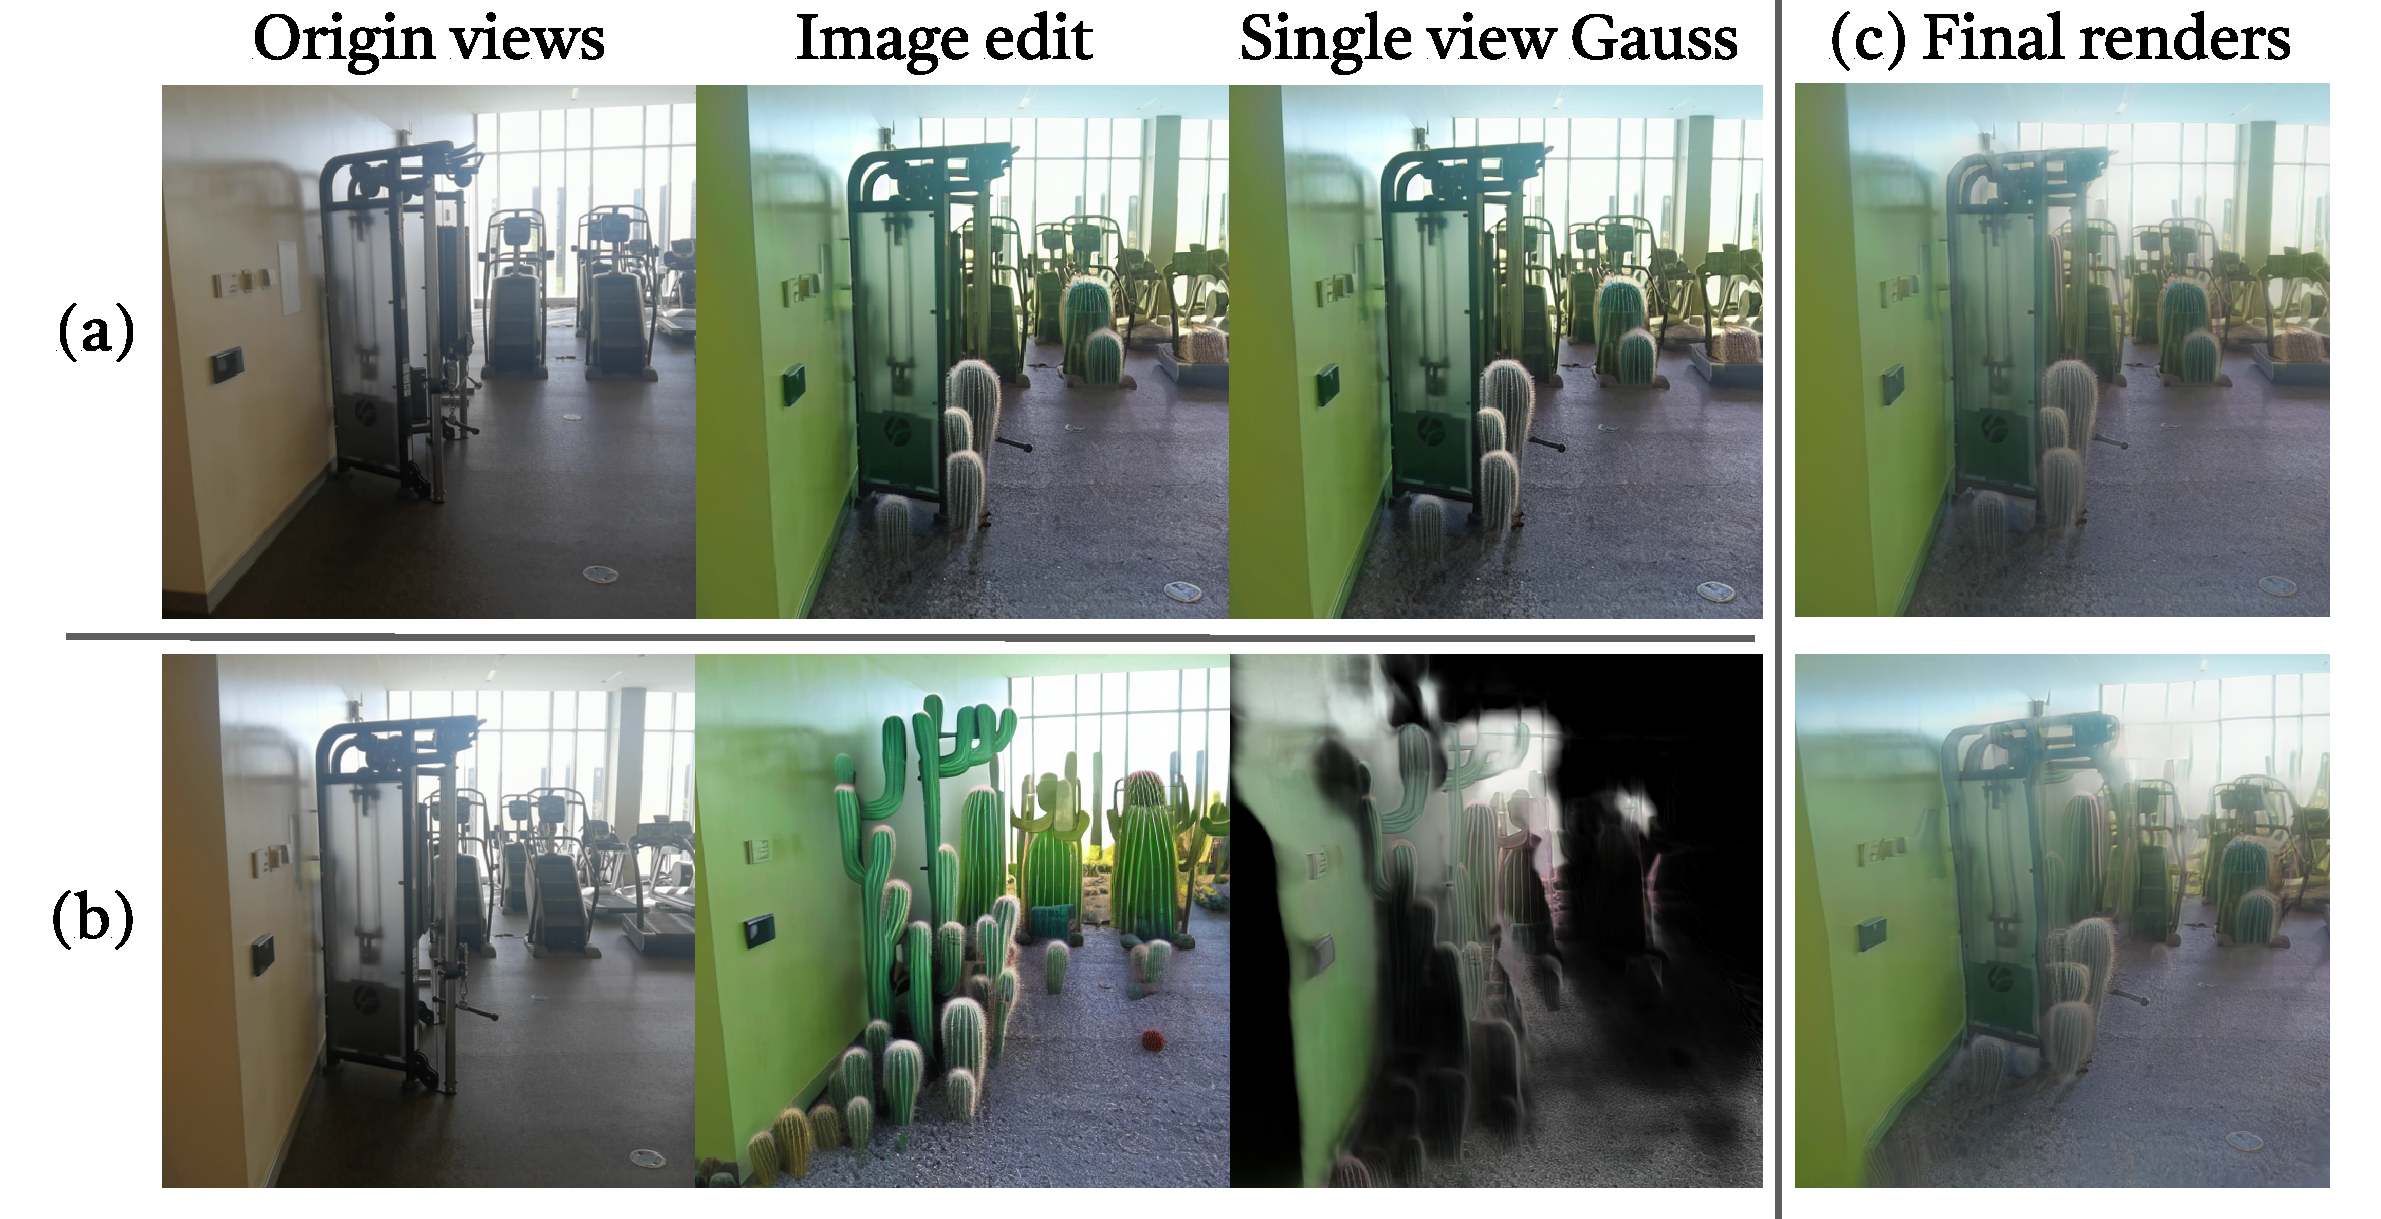
\includegraphics[width=\linewidth]{fig/edit_example_v2.pdf}  
    \caption{\textbf{Example of inference-time editing.}
    (a) First input view, its edited result, and the corresponding single-view Gaussian rendering.
    (b) Second input view, its edited result, and the corresponding single-view Gaussian rendering.
    (c) Final rendering obtained by combining Gaussians from both views. \textit{Prompt: Add a cactus garden.}}
    \label{fig:edit_example}
    \vspace{-2mm}
\end{figure}
\subsection{Inference}
Although our model is trained solely on recolored images, it generalizes effectively to images edited by various 2D editing methods~\cite{ip2p, labs2025flux1kontextflowmatching}.  
Unlike optimization-based pipelines that require iterative test-time fitting, inference in our system is fully feed-forward.  
Since the 2D editing stage operates independently from both the feed-forward reconstruction and the training procedure, our approach is highly flexible and can accommodate diverse image editing techniques~\cite{gpt4o, labs2025flux1kontextflowmatching, geminiteam2025geminifamilyhighlycapable}.  
For experiments and evaluations, we primarily employ commonly used IP2P~\cite{ip2p} as the 2D editor, while additional editors are included in ablation studies.  

As illustrated in Fig.~\ref{fig:teaser}, given a multi-view sequence \(\{I_v\}_{v=0}^{V-1}\) and a text instruction \(\mathcal{E}\), we first generate per-frame edited images \(\{I_v^\star\}_{v=0}^{V-1}\) with a 2D image editor.  
This differs from the training setup, where only the first frame is edited; at inference, all frames are edited to maximize cross-view evidence.  
We then perform a single feed-forward pass of {\ourmethod} to produce the edited 3D Gaussians and render novel views.
Fig.~\ref{fig:edit_example} provides a more concrete example: we visualize the Gaussians generated from the two input views separately in (a) and (b). 
Due to the inconsistency introduced by the 2D image editor, pixels in the second view can conflict with those in the first view; in these regions, the Gaussians from the second view automatically reduce their opacity to mitigate the conflict. 
Panel (c) shows the final rendering obtained by combining the Gaussians from both views, demonstrating view-consistent results.

\subsection{DL3DV-Edit-Bench}
\vspace{1mm}
\noindent\textbf{Motivation and Scope.}
Most existing 3D editing evaluations~\cite{in2n} either focus on single-object or toy scenes rather than full scene editing (\eg, limited context and occlusions), or rely on ad-hoc, privately curated data without a standardized protocol. This hampers fair comparison: methods differ in scene diversity, edit categories, and evaluation criteria. 
We therefore build \textbf{{\ourbench}} on top of the DL3DV~\cite{ling2023dl3dv10klargescalescenedataset} test split, covering diverse indoor/outdoor real scenes and four text-driven edit types: \emph{Add}, \emph{Remove}, \emph{Modify} (attribute/material/appearance), and \emph{Global} (style/exposure). The benchmark targets \emph{scene-level} editing under multi-view inputs and measures both edit effectiveness and cross-view consistency in realistic settings.

\vspace{1mm}
\noindent\textbf{Generation Pipeline.}
We start from the DL3DV test set and sample $20$ real-world scenes (indoor / outdoor). We first run Grounding-DINO~\cite{liu2024groundingdinomarryingdino} on all views to obtain object-level labels and region proposals. The per-scene image set and extracted labels are then fed to a large language model to synthesize candidate prompts for the four edit categories (Add / Remove / Modify / Global). 
We manually vet and keep $5$ valid prompts per scene, resulting in $100$ total edit instances. To ensure multi-view consistency during editing, we fix the 2D image editor, \emph{share} the same random seed and textual prompt across all views of a scene, and confine local edits with masks derived from the proposals. All editor hyperparameters (CFG, steps, strength schedule) are documented and kept constant unless otherwise stated.

\section{Experiments}

\subsection{Implementation Details}
Our main experiments are conducted on the {\ourbench} that we curate to serve as our primary evaluation benchmark. 
% To align with prior work, we additionally report results on the public datasets used in those papers in the appendix. 
For the 2D image-editing module, we use InstructPix2Pix~\cite{ip2p} as the default editor to ensure comparability, and we evaluate more editors in ablations. All experiments are run on a single NVIDIA RTX 6000 GPU.


\subsection{Baselines}
We compare against three methods: (1) EditSplat~\cite{lee2025editsplatmultiviewfusionattentionguided} (optimization-based) with its original 2D editor, InstructPix2Pix, kept unchanged to avoid re-tuning and ensure fairness; (2) GaussCtrl~\cite{gaussctrl} (optimization-based) likewise retaining the authors’ ControlNet module. Both optimization-based baselines are compute-intensive and, in addition to the text prompt, require a pre-reconstructed DL3DV scene, which we supply from standardized baseline reconstructions for parity. (3) NoPoSplat~\cite{noposplat} (feedforward-based), which runs the released checkpoint and consumes only the multi-view inputs for reconstruction, serving as a lower bound on cross-view edit consistency and isolating the contribution of our cross-view fusion in the feed-forward design.

\begin{figure*}[t]
    \centering
    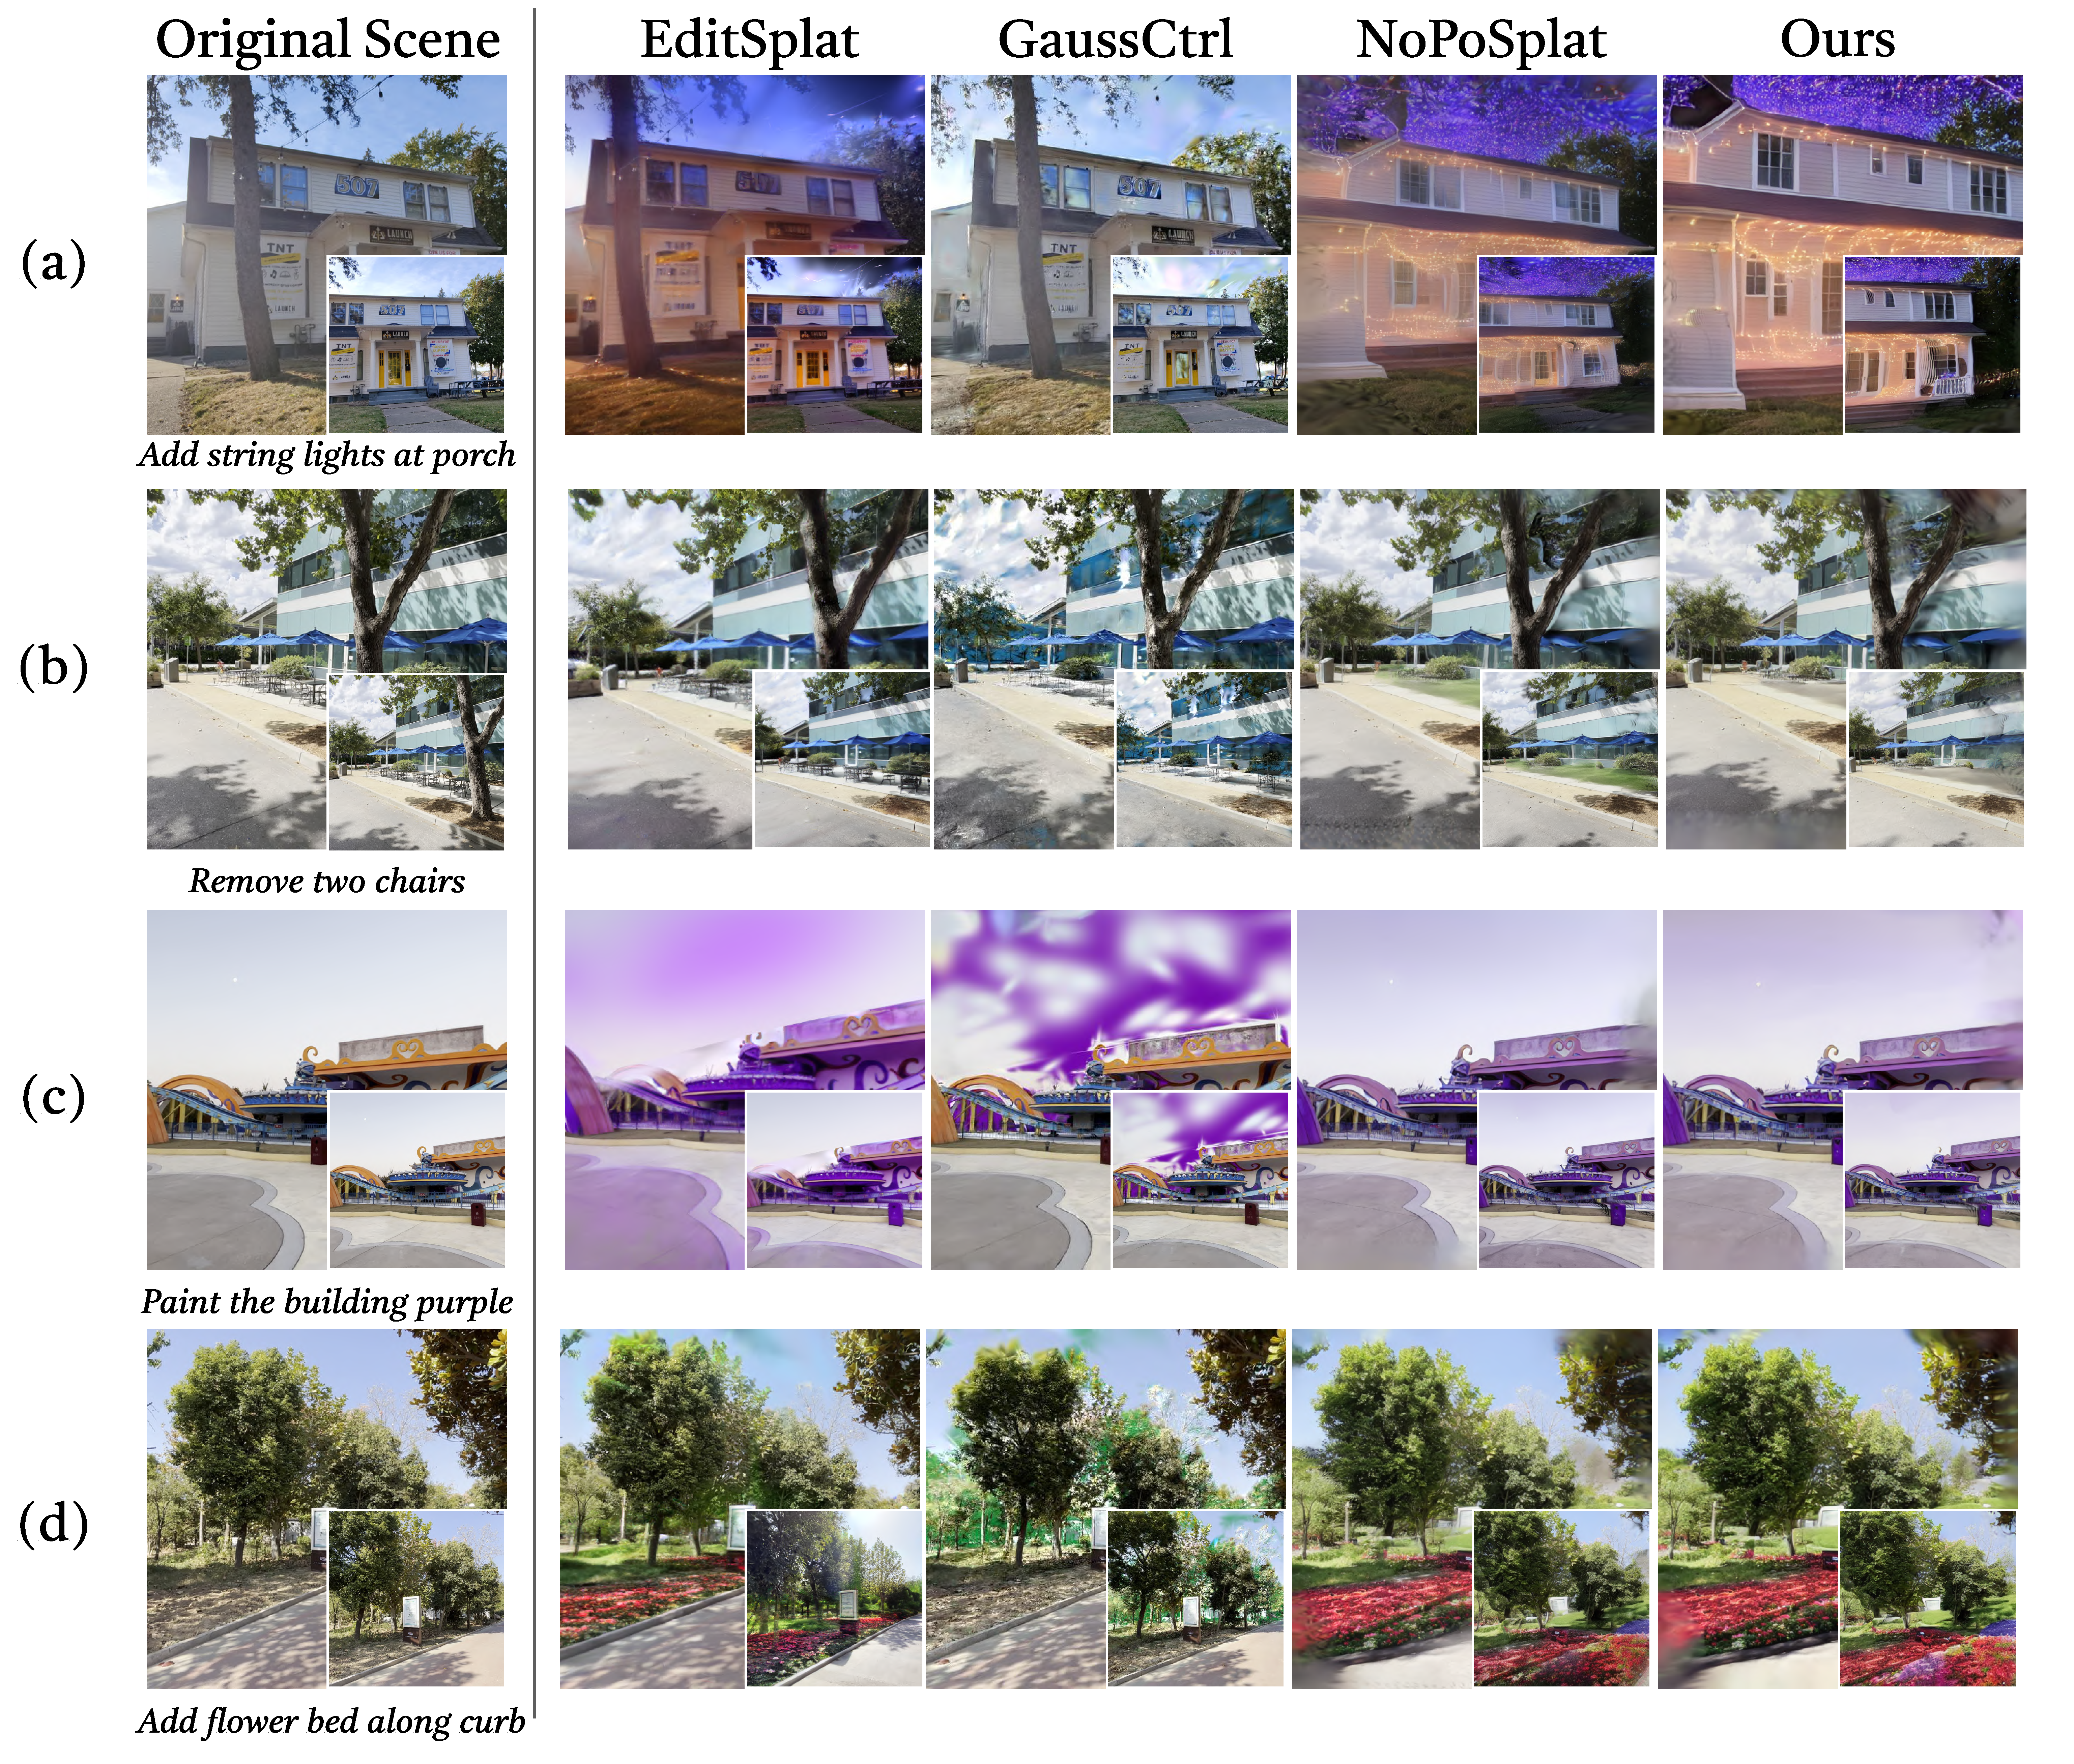
\includegraphics[width=0.93\textwidth]{fig/qualitative_comparison_v4.pdf}
    \caption{\textbf{Qualitative comparison} among four methods. The first row shows the original scene and the editing prompt; the remaining four rows show the results, each paired with an additional view.}
    \label{fig:qualitative-examples}
\end{figure*}

\subsection{Main Experiments} 
\vspace{1mm}
\noindent\textbf{Evaluation Metrics.} Similar to prior works~\cite{lee2025editsplatmultiviewfusionattentionguided, gaussctrl, in2n, you2025instainpaintinstant3dsceneinpainting}, we evaluate effectiveness from two angles: (1) whether the method performs the intended scene edits; (2) whether the 3D reconstruction is plausible across viewpoints. For (1), acknowledging the subjectivity of 3D scene generation, we adopt CLIP~\cite{radford2021learningtransferablevisualmodels} image-text similarity, which scores the absolute alignment between the edited render and the target description. For (2), we report C-FID~\cite{heusel2018ganstrainedtimescaleupdate}, which measures distribution-level realism by computing the Fréchet distance between feature distributions of edited renders and reference views, and C-KID~\cite{bińkowski2021demystifyingmmdgans}, which measures the kernel MMD between the same feature distributions and is more reliable with moderate sample sizes. Here, the prefix "C-" indicates that both metrics are computed in a scene-conditioned manner. Together they quantify overall realism/naturalness across views.

\vspace{1mm}
\noindent\textbf{Quantitative Comparison.} As summarized in Tab.~\ref{tab:main}, {\ourmethod} achieves the best quality-speed trade-off.
%
In terms of runtime, feed-forward methods are dramatically faster than optimization-based ones; 
{\ourmethod} processes a view in 0.51\,s (vs.\ 325.53\text{–}584.46\,s for optimization-based baselines). 
{\ourmethod} also attains the highest CLIP$_{t2i}$(text prompts to rendered images), indicating stronger instruction following and more effective scene edits. 
By design, GaussianCtrl applies only minor modifications, which keeps outputs close to the original and thus boosts C-FID and C-KID, but it underperforms on text alignment due to limited edit strength. 
EditSplat makes moderate edits and is relatively stable, yet remains conservative overall. 
NoPoSplat focuses on reconstruction rather than explicit editing; when input views are inconsistent, it tends to average conflicting evidence, producing blurred renders and uniformly lower scores (CLIP$_{t2i}$, C-FID and C-KID). 
Overall, {\ourmethod} best balances instruction following with multi-view realism, improving C-FID and C-KID over other feed-forward baselines while preserving semantics and structure nearly as well as the most conservative optimizer.

\vspace{1mm}
\noindent\textbf{Qualitative Comparison.}
Fig.~\ref{fig:qualitative-examples} presents four examples (a–d) of scene editing by EditSplat~\cite{lee2025editsplatmultiviewfusionattentionguided}, GaussCtrl~\cite{gaussctrl}, NoPoSplat~\cite{noposplat}, and {\ourmethod}. The small inset at the bottom-right of each panel shows the result from another viewpoint of the same scene. EditSplat achieves partially successful edits in (a, c, d), but it also alters regions that should remain unchanged, such as the sky and ground in (c). GaussCtrl is almost entirely unsuccessful across (a–d), producing chaotic or ineffective edits when applied to scenes that are unseen during its training. NoPoSplat generally generates plausible results, but its quality is highly sensitive to the inconsistency between input views: when cross-view inconsistency is large, it suffers from blur in (a,d), whereas for more consistent inputs in (b,c), the reconstruction quality is much better. In contrast, our method delivers stable, high-quality edits across all four scenes, maintaining consistency across views while preserving the original scene structure.

\begin{table}[t]
\centering
\scriptsize
\caption{\textbf{Quantitative comparison} on optimization-based and feed-forward methods.}
\label{tab:main}
\setlength{\tabcolsep}{6pt}
\renewcommand{\arraystretch}{1.1}
% \resizebox{\textwidth}{!}{%
\begin{tabular}{l@{\hskip 1.0mm}l@{\hskip 1.0mm}c@{\hskip 1.0mm}c@{\hskip 1.0mm}c@{\hskip 1.0mm}c}
\toprule
\textbf{Category} & \textbf{Method} &
\textbf{Time (s)}\,(\(\downarrow\)) &
\text{CLIP}$_{t2i}$(\(\uparrow\)) &
\textbf{C-FID}\,(\(\downarrow\)) &
\textbf{C-KID}\,(\(\downarrow\)) \\
\midrule
\multirow{2}{*}{Optimization}
& GaussCtrl~\cite{gaussctrl} & 325.53 & 0.227 & 135.0 & 0.091 \\
& Editsplat~\cite{lee2025editsplatmultiviewfusionattentionguided} & 584.46 & 0.241 & 174.1 & 0.122 \\
\midrule
\multirow{2}{*}{Feed-forward}
& NoPoSplat~\cite{noposplat} & 0.61   & 0.253 & 180.6 & 0.125 \\
& {\ourmethod} (Ours)   & 0.51   & 0.266 & 171.3 & 0.116 \\
\bottomrule
\vspace{-4mm}
\end{tabular}%
% }
\end{table}


\begin{table}[t]
\centering
\scriptsize
\caption{\textbf{Ablation quantitative comparison} on different training strategies in our method.}
\label{tab:training_ablation}
\setlength{\tabcolsep}{6pt}
\renewcommand{\arraystretch}{1.1}
\begin{tabular}{l@{\hskip 8.0mm}c@{\hskip 8.0mm}c@{\hskip 8.0mm}c}
\toprule
\textbf{Method} & \textbf{CLIP$_{t2i}$~(\(\uparrow\))} &
\textbf{C-FID~(\(\downarrow\))} & \textbf{C-KID~(\(\downarrow\))} \\
\midrule
{\ourmethod}  & 0.266 & 171.3 & 0.116 \\
+w/o Recolor   & 0.243 & 215.0 & 0.141 \\ %场景出现模糊
+w/o 3D Loss   & 0.237 & 278.4 & 0.182 \\ %场景歪的非常厉害
+w/o SAM  & 0.248 & 179.6 & 0.127 \\ %表现略微下降
+w/o R-Drop & 0.252 & 183.1 & 0.130 \\ %场景出现歪，深度出问题，view差距大了会出错，表现几乎不变
\bottomrule
\vspace{-4mm}
\end{tabular}
\end{table}

\subsection{Ablation Study}
We validate our design choices by comparing {\ourmethod} against different training and inference variants. Unless otherwise stated, the default configuration uses SAM2-based recoloring for supervision, the asymmetric input scheme, our full training losses (2D appearance + 3D regularization), randomly dropping the first view's Gaussian with $p{=}0.5$ during training; and InstructPix2Pix as the editing front-end at inference.

\vspace{1mm}
\noindent\textbf{Recolor/Image Editing For Training.}
Directly training on multi-view images produced by a 2D editor inevitably introduces substantial cross-view inconsistencies that act as label noise and hinder convergence. We therefore supervise training with \emph{SAM2-based recoloring}: object masks are extracted and recolored consistently across views, yielding stable, view-aligned targets. As Table \ref{tab:training_ablation} shows, in our ablations, replacing recoloring data with direct multi-view editing degrades multi-view consistency and increases artifacts, confirming the need for view-consistent supervision.

\vspace{1mm}
\noindent\textbf{Training Loss.} 
Because recoloring/editing can shift predicted Gaussian centers, relying solely on 2D losses (reconstruction/style) permits geometry drift: the rendering may look plausible while Gaussian primitives misalign in 3D. We ablate our 3D regularizers, and results are shown in Tab.~\ref{tab:training_ablation} . Removals lead to larger center deviation and diminished cross-view coherence. Using the full loss stabilizes geometry and improves semantic fidelity without sacrificing appearance.

\vspace{1mm}
\noindent\textbf{SAM2 Segmentation For Augmentation.}
To narrow the distribution gap between recolored training images and edited images at inference, we augment training data with SAM2-derived mask jittering (dilation/erosion), palette perturbation, and limited background leakage. Ablating these SAM2-based augmentations by training with plain recoloring only, reduces robustness and increases failure cases under stronger edits, indicating that modest variability during training is beneficial. Results are shown in Tab.~\ref{tab:training_ablation}.

\vspace{1mm}
\noindent\textbf{Random Drop the First View's Gaussian.}
Given the asymmetric inputs, the edited reference view can dominate the learned style. We introduce random drop during training: with probability $0.5$, we discard the Gaussians associated with the first view when forming supervision, forcing the network to propagate the edit semantics from the reference to the auxiliaries. Ablations on the drop probability, results in Tab.~\ref{tab:training_ablation}, show that removing random drop causes overfitting to the reference viewpoint, while excessively high drop rates weaken edit strength.

\begin{figure}[t]  % [t] 顶端
\scriptsize
    \centering
    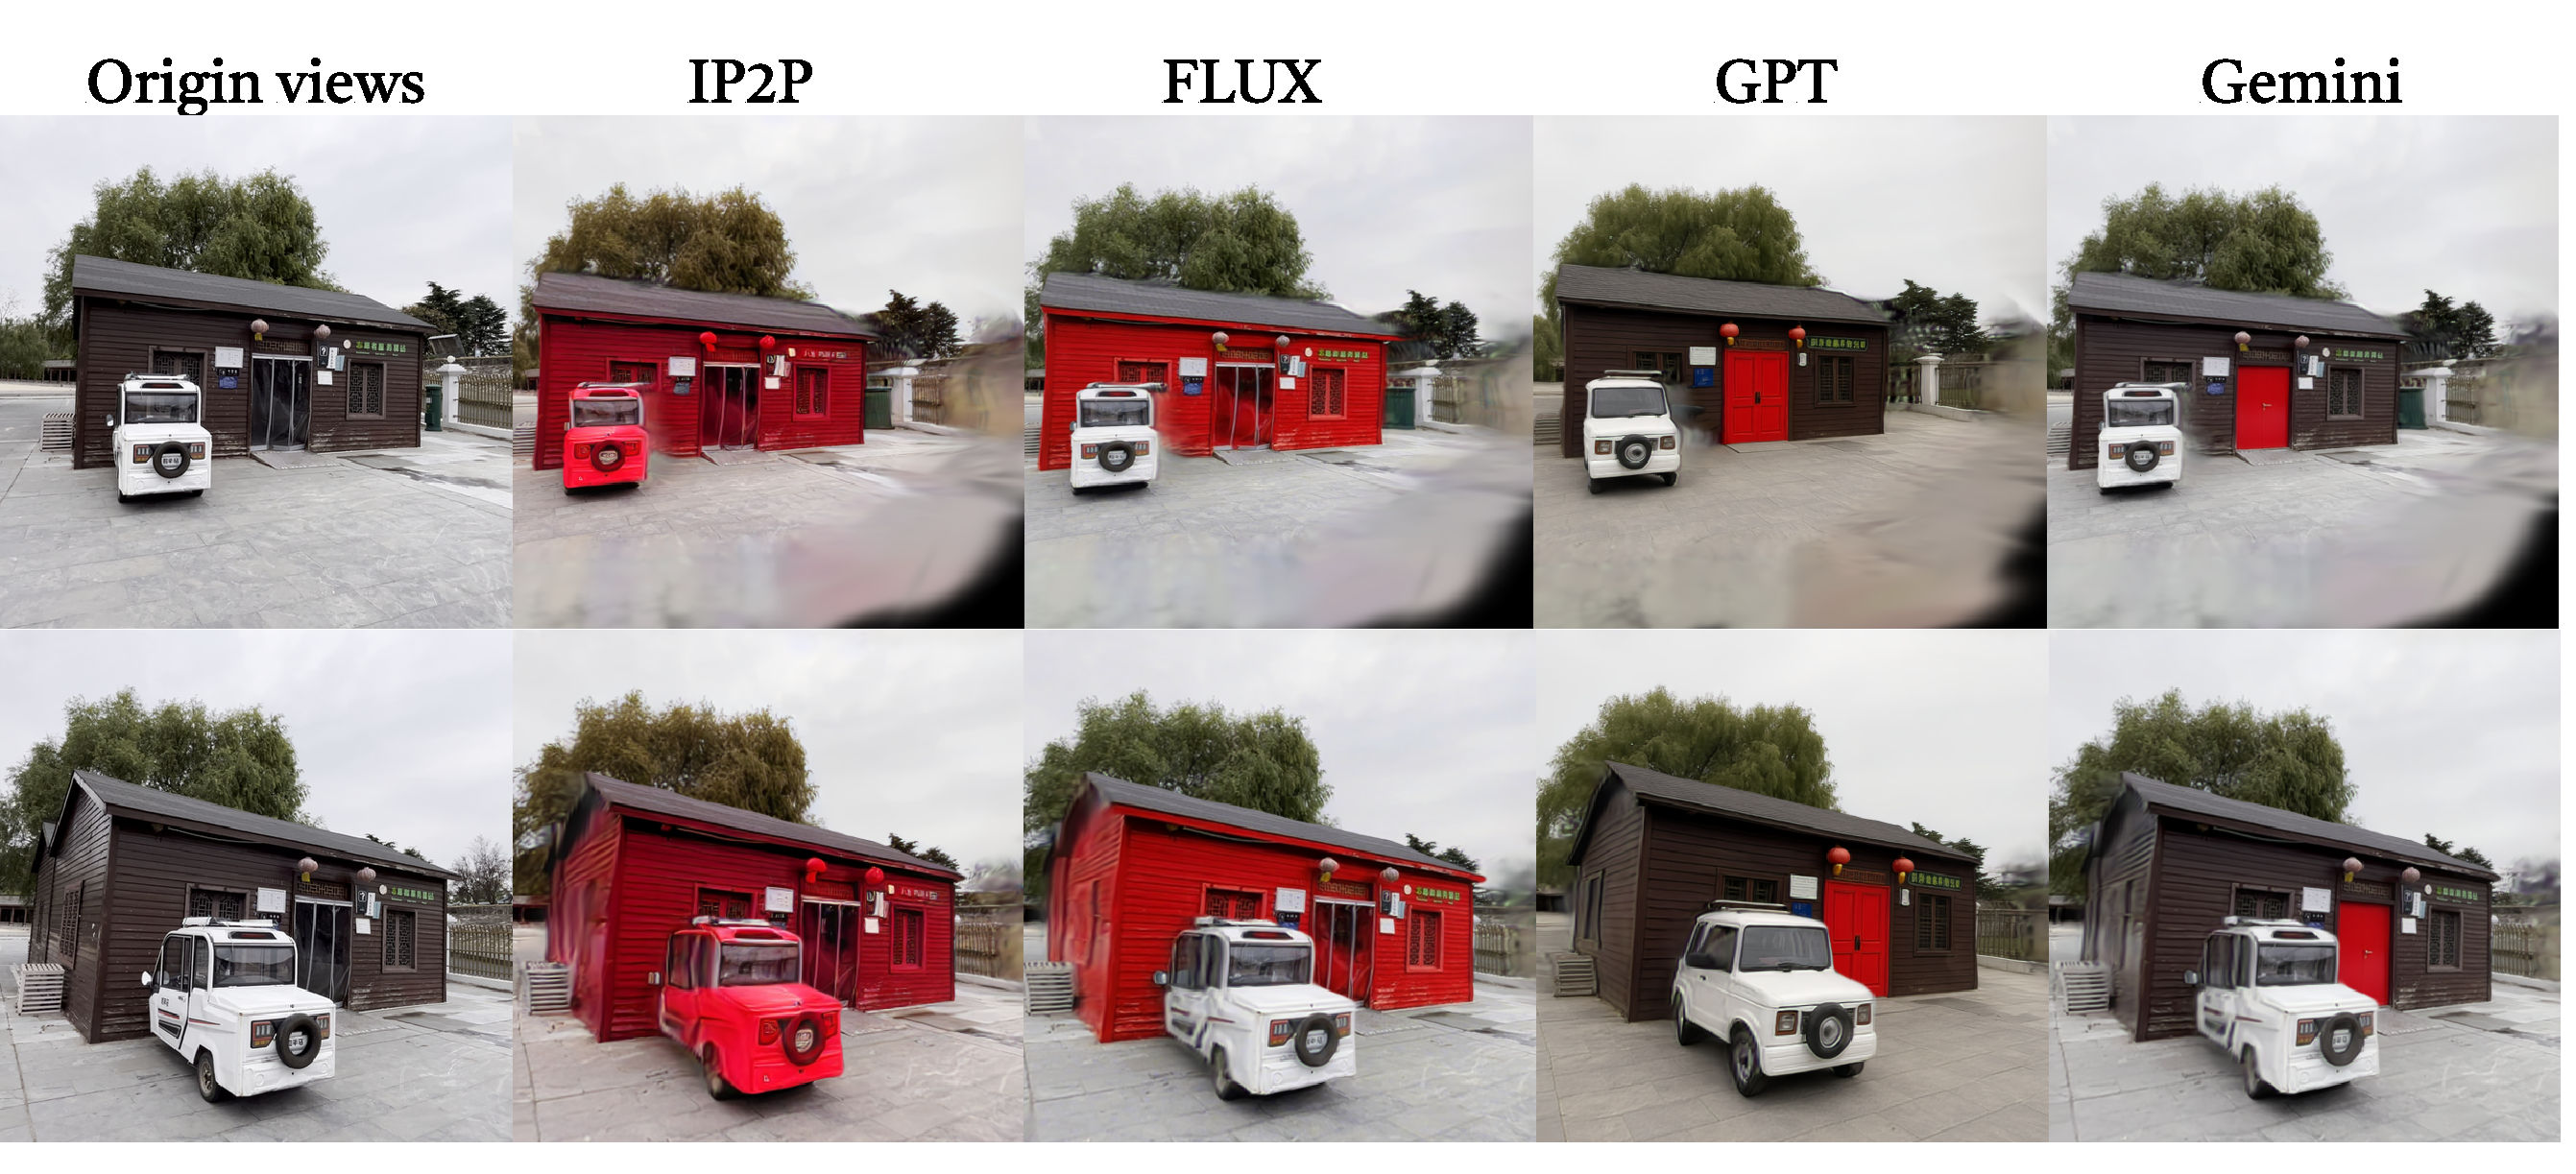
\includegraphics[width=\linewidth]{fig/image_editor.pdf}
    \caption{\textbf{Ablation qualitative comparison} among four image editors. \textit{Prompt: Paint the door red.}}
    \label{fig:image-editor}
    \vspace{-4mm}
\end{figure}

\vspace{1mm}
\noindent\textbf{Image Editing For Inference.}
Our pipeline decouples 2D editing from feed-forward reconstruction, allowing different editors at test time. We evaluate IP2P~\cite{ip2p} and alternatives including (1) OpenAI GPT-Image-1~\cite{gpt4o} (GPT) (2) Google Gemini-2.5-Flash-Image~\cite{geminiteam2025geminifamilyhighlycapable} (Gemini) (3) FLUX~\cite{labs2025flux1kontextflowmatching}. 
As shown in Fig.\ref{fig:image-editor} and Tab.\ref{tab:image_editor}, FLUX produces the highest visual edit quality but its edited regions are sometimes mislocalized; GPT and Gemini accurately identify the intended edit regions but tend to modify other parts of the image, while IP2P yields weak perceptual edit quality among the four.
Across editors, {\ourmethod} preserves its advantages in speed and consistency; stronger editors can improve local edit quality, while our model continues to enforce cross-view coherence. This indicates that {\ourmethod} is editor-agnostic and can benefit from future improvements in 2D editing.

\begin{table}[t]
\centering
\scriptsize
\caption{\textbf{Ablation quantitative comparison} on different image editors in our method.}
\vspace{-2mm}
\label{tab:image_editor}
\setlength{\tabcolsep}{6pt}
\renewcommand{\arraystretch}{1.1}

\begin{tabular}{l@{\hskip 8.0mm}c@{\hskip 8.0mm}c@{\hskip 8.0mm}c}
\toprule
\textbf{Method} & \textbf{CLIP$_{t2i}$~(\(\uparrow\))} &
\textbf{C-FID~(\(\downarrow\))} & \textbf{C-KID~(\(\downarrow\))} \\
\midrule
IP2P~\cite{ip2p}  & 0.266 & 171.3 & 0.116 \\
GPT~\cite{gpt4o}    & 0.261 & 166.2 & 0.102 \\ Gemini~\cite{geminiteam2025geminifamilyhighlycapable}  & 0.246 & 150.3 & 0.098 \\
FLUX~\cite{labs2025flux1kontextflowmatching}  & 0.276 & 169.9 & 0.112 \\
\bottomrule
\end{tabular}
\vspace{-4mm}
\end{table}
%
\section{Conclusion}
We introduced \ourmethod, a pose-free, feed-forward framework that unifies reconstruction and instruction-driven editing of 3D scenes from unposed, instruction-edited images. By directly predicting edited 3D Gaussian splats in a single pass—without test-time optimization or pose estimation—our approach departs from the conventional reconstruct-edit-refit pipeline and enables fast, photorealistic, and instruction-aligned rendering. Two design choices are key to making this practical at scale: (i) a SAM2-based recoloring strategy that provides reliable, cross-view-consistent supervision despite the lack of true multi-view edited ground truth; and (ii) an asymmetric input scheme that pairs an edited reference view with unedited auxiliary views, encouraging the network to fuse disparate observations while preserving scene structure. Coupled with lightweight 3D regularization on Gaussian centers, these components yield robust multi-view coherence even when the input edits are imperfect or inconsistent.

To enable fair and reproducible comparisons, we proposed {\ourbench}, a scene-level benchmark spanning 20 diverse scenes and four edit types (Add / Remove / Modify / Global). On this benchmark, {\ourmethod} achieves stronger text-image alignment and improved 3D consistency than recent optimization-based and feed-forward baselines, while being orders of magnitude faster at inference. Ablations confirm the necessity of view-consistent recoloring, asymmetric inputs, and 3D geometric losses, and demonstrate that our method is editor-agnostic and generalizing to a range of 2D editing front-ends.

\vspace{1mm}
\noindent\textbf{Limitations and Future Work.}
Although recoloring provides stable supervision, it does not fully capture large geometric changes (\eg, substantial add/remove edits) or extreme material and illumination shifts. Looking ahead, promising directions include expanding supervision beyond recoloring with view-consistent generative augmentation, learning per-object disentangled controls for precise 3D edits, incorporating uncertainty-aware rendering to handle ambiguous or conflicting edits, extending to dynamic scenes and longer view sequences, and further enriching {\ourbench} with more diverse and complex scenes.


% Although recoloring offers stable supervision, it underrepresents large geometric changes (\eg, substantial add / remove edits) and extreme material / illumination shifts. Future directions include: 
% scaling supervision beyond recoloring via view-consistent generative augmentation; learning per-object, disentangled controls for precise 3D edits; 
% incorporating uncertainty-aware rendering to handle ambiguous or conflicting edits; 
% extending to dynamic scenes and longer view sequences; 
% and broadening {\ourbench} with richer scenes, stronger metrics, and human studies.
% \clearpage
\setcounter{page}{1}


\twocolumn[{% 
\renewcommand\twocolumn[1][]{#1}% 
\maketitlesupplementary
\begin{center} 
% \vspace{-0.2in}
\vspace{8mm}
\centering 
\includegraphics[width=\textwidth]{fig/Supp_pipeline.pdf}
    \captionsetup{width=\linewidth}
    \captionof{figure}{\textbf{\ourmethod} Backbone pipeline.}
    \label{fig:edit3r-arch}
    \vspace{4mm}
\end{center}
}]

\section{Method \& Architecture Details}
\label{sec:arch}
\subsection{Detailed Structure}

Figure~\ref{fig:edit3r-arch} illustrates the network architecture of {\ourmethod}.
Our model is built upon the pose-free large reconstruction model NoPoSplat~\cite{noposplat} and follows the same encoder--decoder--head design, while adapting it to asymmetric edited inputs for 3D scene editing.

\paragraph{Inputs and tokenization.}
Given two unposed RGB views and their camera intrinsics
\(\{(I'_0, k_0), (I_1, k_1)\}\),
where \(I'_0\) is the recolored (edited) reference view and \(I_1\) is an unedited auxiliary view,
our goal is to predict a single canonical 3D Gaussian scene that represents the edited content.
Each image is resized and patchified, and a Vision Transformer (ViT)~\cite{vit} encoder operates on the resulting sequence of image tokens.
Following NoPoSplat~\cite{noposplat}, we embed the intrinsics \(k_v\) of each view with a small MLP
\(\phi: \mathbb{R}^d \rightarrow \mathbb{R}^D\) and append the resulting \emph{intrinsics token} to the image tokens:
\begin{equation*}
    z_v = \big[\,\text{img\_tokens}(I_v) \oplus \phi(k_v)\,\big],
\end{equation*}
This intrinsic-token strategy improves scale stability and removes the need for pose supervision, as observed in~\cite{noposplat}.

\paragraph{Shared ViT encoder.}
The two views are processed independently by a shared-weight ViT encoder.
For each view \(v\), the encoder produces a sequence of latent tokens
\(f_v\) at a constant spatial resolution (downsampled with respect to the input image).
At this stage, the views do not interact; each \(f_v\) encodes high-level appearance and coarse geometry for its corresponding image.

\paragraph{Multi-view ViT decoders with cross-attention.}
To fuse information across views, {\ourmethod} employs two identical ViT decoders, one per view, that communicate via cross-attention (Fig.~\ref{fig:edit3r-arch}).
Each decoder takes the encoder features \(f_v\) as input and consists of a stack of transformer blocks.
Within each block, self-attention is applied to tokens from a single view, while a cross-attention layer lets tokens from one view attend to tokens from the other view.
In the two-view setting, this yields two decoder branches with shared parameters, where features for \(I'_0\) and \(I_1\) are refined jointly.
This design allows the model to resolve occlusions and reconcile the potentially inconsistent appearance between the edited reference view and the unedited auxiliary view, while still preserving view-specific details.

\paragraph{DPT-based Gaussian prediction heads.}
From the fused decoder features, {\ourmethod} predicts per-pixel Gaussian parameters using two dense prediction heads per view, both based on the DPT architecture~\cite{dust3r}. For view \(v\), let \(f_{fused-v}\) denote the output of the ViT decoder.

\begin{itemize}
    \item \textbf{Center head.}
    The \emph{center head} takes only \(f_{fused-v}\) as input and upsamples it via a DPT-style decoder to full image resolution.
    It regresses a 3D center \(\boldsymbol{\mu} \in \mathbb{R}^3\) for each pixel, yielding a dense field of Gaussian centers in a canonical world frame.

    \item \textbf{Parameter head.}
    The \emph{parameter head} predicts the remaining Gaussian attributes.
    It receives both the decoder features and a high-resolution RGB shortcut from the corresponding input image:
    \begin{equation}
        \mathbf{H}_v = \mathrm{concat}\!\big(f_{fused-v}, \mathrm{RGB\_feat}(I_v^{\mathrm{RGB}})\big),
    \end{equation}
    where \(I_v^{\mathrm{RGB}}\) is \(I'_0\) for the edited reference branch and \(I_1\) for the auxiliary branch.
    A DPT decoder processes \(\mathbf{H}_v\) and predicts opacity \(\alpha\), anisotropic covariance parameters (orientation and scale), and low-order spherical-harmonic color coefficients \(c\) for each pixel.
    The RGB shortcut compensates for the lower spatial resolution of ViT features and is crucial for recovering fine-grained textures and edges, as also reported in~\cite{noposplat}.
\end{itemize}

For each pixel in each view we thus obtain a Gaussian
\(({\mu}_j, {\Sigma}_j, \alpha_j, c_j)\).
All Gaussians are expressed directly in the canonical coordinate system and do not require any explicit pose estimation or local-to-global transformation.

\paragraph{Canonical-space fusion and rendering.}
The Gaussian primitives from the two branches are concatenated to form a single set
\(\mathcal{G} = \{(\mu_j, \Sigma_j, \alpha_j, c_j)\}\)
representing the edited 3D scene.
We render \(\mathcal{G}\) using standard 3D Gaussian splatting to obtain supervision views during training (recolored targets) and novel edited views at inference time.
Because the two decoder branches share weights and interact via cross-attention, {\ourmethod} learns to fuse the edited reference view and the unedited auxiliary view into a coherent 3D representation, even when the 2D edits are view-inconsistent.

\paragraph{Differences from NoPoSplat.}
Architecturally, {\ourmethod} reuses the NoPoSplat backbone (ViT encoder, multi-view ViT decoder with cross-attention, and DPT center/parameter heads) but changes the input configuration and training objectives.
The encoder--decoder now receives an \emph{asymmetric} pair of images \((I'_0, I_1)\), and the RGB shortcuts for the parameter heads are taken from the edited and unedited images, respectively.
Combined with our SAM2-based recoloring, asymmetric input scheme, and 3D regularization losses, this architecture enables {\ourmethod} to map view-inconsistent 2D edits to a single, view-consistent set of 3D Gaussians while retaining the fast, feed-forward inference of the original pose-free reconstructor.

\subsection{Training Loss Detail}
During training, our model is optimized with a combination of 2D appearance losses and 3D geometric regularizers, applied to every supervision view. Given the rendered prediction $\hat{I}_v$ for view $v$ and its corresponding ground-truth image $I_v$, we minimize a weighted sum of a CLIP-based semantic loss, a perceptual LPIPS loss, and a low-frequency MSE loss over all views, together with two 3D losses that regularize the predicted Gaussian scene structure. Formally, the total loss can be written as
\begin{equation*}
\begin{split}
\mathcal{L}_{\text{total}}
= \sum_{v} \Big(
\lambda_{\text{CLIP}} \mathcal{L}_{\text{CLIP}}(\hat{I}_v, I_v)
+ \lambda_{\text{LPIPS}} \mathcal{L}_{\text{LPIPS}}(\hat{I}_v, I_v)\\
+ \lambda_{\text{MSE}} \mathcal{L}_{\text{MSE}}(\hat{I}_v, I_v)
\Big)
+ \lambda_{\text{center}} \mathcal{L}_{\text{center}}
+ \lambda_{\text{geom}} \mathcal{L}_{\text{geom}}.
\end{split}
\end{equation*}
As mentioned in the main paper, the scalar weights $\lambda_{\cdot}$ correspond to the configuration weights of each loss module, with $\lambda_{\text{CLIP}} = 0.5$, $\lambda_{\text{LPIPS}} = 0.8$, $\lambda_{\text{MSE}} = 1.0$, $\lambda_{\text{center}} = 0.01$, and $\lambda_{\text{geom}} = 0.03$.


\begin{figure*}[t]
    \centering
    \includegraphics[width=\textwidth]{fig/Supp_sam.pdf}
    \caption{\textbf{SAM2 segmentation detailed pipeline.}}
    \label{fig:supp_sam}
\end{figure*}

\subsection{SAM2 Configuration and Usage}
\label{sec:sam2_supp}

We adopt the official SAM2 implementation with the \texttt{sam2.1\_hiera\_small} checkpoint and use it in two stages: (i) object discovery on the first frame, and (ii) mask propagation over the entire video. Concretely, we instantiate a \texttt{SAM2AutomaticMaskGenerator} with the following hyperparameters:
\begin{itemize}
    \item \texttt{points\_per\_side} $= 32$,
    \item \texttt{pred\_iou\_thresh} $= 0.7$,
    \item \texttt{stability\_score\_thresh} $= 0.92$,
    \item \texttt{crop\_n\_layers} $= 1$,
    \item \texttt{crop\_n\_points\_downscale\_factor} $= 2$,
    \item \texttt{min\_mask\_region\_area} $= 100$.
\end{itemize}
On the first frame of each sequence, the automatic mask generator proposes candidate regions. We then apply the deterministic multi-criterion filter defined in the main paper: a mask is kept only if (i) its area $A$ is at least
$A_{\min} = 400$ pixels, (ii) its stability score $s$ satisfies
$s \geq s_{\min} = 0.92$, (iii) its predicted IoU $q$ satisfies
$q \geq q_{\min} = 0.7$, (iv) the aspect ratio of its bounding box
$r = w/h$ lies in $[r_{\min}, r_{\max}] = [0.1, 10]$ (to avoid
extremely thin or flat regions), and (v) its bounding box has at least
$m_{\text{edge}} = 10$ pixels of margin to the image boundary on all sides.
The remaining instances are sorted by area, and we retain at most $N_{\max} = 20$ objects per sequence.

For temporal tracking, we use the SAM2 video predictor. We first initialize an internal inference state on the extracted frame sequence and then add each selected mask on the first frame as a separate object ID. We run the built-in \texttt{propagate\_in\_video} routine to obtain per-frame mask logits for each object; logits are binarized at zero to produce final foreground masks. To suppress identity drift, we compare the set of active object IDs in each frame to that of the most recently accepted frame and discard a frame if the size of their intersection is smaller than $0.5$ times the larger of the two set cardinalities. Such frames are excluded from subsequent processing (including our recoloring and supervision stages).

An example of this pipeline is visualized in Fig.~\ref{fig:supp_sam}. For each video, SAM2 first performs object-level segmentation on the initial frame and returns up to 20 candidate masks (three of which are shown). These selected masks are then propagated to subsequent frames by the video predictor, which maintains object identities over time and yields temporally consistent foreground masks. Applying our recoloring procedure to each frame based on these propagated masks produces coherent multi-frame edits.


\subsection{3D Regularization}
\begin{figure}
\scriptsize
    \centering
    \includegraphics[width=\linewidth]{fig/Supp_3Dloss.pdf}
    \caption{\textbf{Examples of training results without 3D constraints.}}
    \label{fig:supp_3dloss}
    \vspace{-4mm}
\end{figure}

\paragraph{Motivation.}
Text-driven 2D scene editing inevitably perturbs the appearance and depth cues of the input views in a view-dependent way. In our setting, the underlying scene geometry is expected to remain close to the original reconstruction, but the edited images no longer follow a single, globally consistent depth field. As a consequence, if we only optimize 2D reconstruction losses, the model can fit the edited supervision by sliding Gaussian primitives along the viewing rays: the rendered images still match the edited inputs, but the predicted Gaussian centers drift in depth and the reconstructed surfaces become distorted.
As shown in Fig.\ref{fig:supp_3dloss}(a), when training with 2D losses only, the Gaussians predicted from the two views yield human heads of noticeably different sizes: the Gaussian centers in the edited view are pulled towards the camera in an attempt to cover the content in view2, while the centers in view2, being largely occluded, become unconstrained and drift backwards.
%如图（a）部分所示，在只加2D loss训练的情况下，两个view预测的两个gaussian之间出现了不同大小的人头，gaussian center会出现往镜头方向移动的情况，试图覆盖掉view2，而view2因为被覆盖住了，gaussian center的位置就不受控制了,往后扩大

This issue is further exacerbated by our asymmetric input design, where the edited reference view and the unedited auxiliary view undergo different amounts and patterns of appearance change. The network then tends to explain each view with a different depth configuration, which leads to view-dependent ``layering'' and misalignment of the 3D Gaussians reconstructed from different views. In practice, we observe that, without additional 3D constraints, the same physical surface may be represented by different depth layers in the two views. 
As shown in Fig.\ref{fig:supp_3dloss}(b), training with 2D losses only also causes a layered structure between the Gaussians from view1 and view2, where the Gaussians of view1 are consistently pushed forward along the viewing direction in an attempt to cover those from view2.
%如图（b）所示，在只加2D loss训练的情况下，导致的另一个结果是view1的gaussian和view2的gaussian出现分层的情况，view1会尽量往前把view2覆盖住

\paragraph{3D Loss Design.}
To prevent such degenerate solutions, we introduce two complementary 3D losses. First, we apply a depth/center regularization loss that anchors the edited Gaussians to the reference centers predicted by a frozen LRM on the unedited images. This term constrains the optimization to stay close to the original 3D geometry and avoids large depth shifts caused purely by appearance edits. 

Second, we enforce a multi-view geometric consistency loss that penalizes discrepancies between Gaussian centers inferred from different views, encouraging them to converge to a shared, view-independent configuration.


% \paragraph{CLIP-based semantic loss $\mathcal{L}_{\text{CLIP}}$.}
% The CLIP loss encourages the rendered images to match the target supervision images in a high-level semantic embedding space rather than only at the pixel level. Concretely, we use the image encoder of CLIP ViT-B/32, which is frozen during training. Both the prediction $\hat{I}_v$ and the ground-truth $I_v$ are first clamped to the $[0,1]$ range and preprocessed with the standard CLIP image normalization (bicubic resize to $224 \times 224$, center crop, and channel-wise normalization). We then encode both images with the CLIP image encoder, $\mathrm{encode\_image}(\cdot)$, and L2-normalize the resulting feature vectors. The loss for each view is implemented as
% \begin{equation*}
% \mathcal{L}_{\text{CLIP}}(\hat{I}_v, I_v)
% = 1 - \left\langle f(\hat{I}_v), f(I_v) \right\rangle,
% \end{equation*}
% i.e., one minus the cosine similarity between the predicted and reference CLIP features, averaged over the batch. This term provides a robust global supervision signal that is tolerant to small misalignments and focuses on preserving the semantics and overall style of the edited scene rather than exact pixel values.

% \paragraph{Perceptual LPIPS loss $\mathcal{L}_{\text{LPIPS}}$.}
% The LPIPS loss refines local perceptual quality by comparing deep feature maps extracted from a pretrained VGG network. We use the official LPIPS implementation with the VGG backbone. For each training view, we reshape the predicted and target images to tensors of shape $(N, C, H, W)$ and feed them into LPIPS with its internal channel-wise normalization enabled. The LPIPS distance is then averaged over all images and multiplied by a scalar weight. To avoid destabilizing the early phase of training, we only activate this loss after a specified global step; before that, LPIPS returns zero and does not contribute to the objective. Once activated, $\mathcal{L}_{\text{LPIPS}}$ encourages the rendered images to match the supervision in mid- and high-frequency structures such as edges, textures, and fine details, improving perceptual fidelity beyond what can be achieved with purely pixel-based losses.

% \paragraph{Low-frequency MSE loss $\mathcal{L}_{\text{MSE}}$.}
% Instead of a standard per-pixel MSE loss, we employ a low-frequency MSE defined on spatially downsampled ``color blocks'' of the images. For each prediction--target pair, we first collapse the view dimension (if present) and obtain tensors of shape $(N, C, H, W)$. We then apply average pooling with a configurable block size $k$ (default $k = 8$). When $H$ and $W$ are divisible by $k$, we use standard average pooling with kernel and stride equal to $k$; otherwise, we apply adaptive average pooling to the largest grid of pooled cells that fits within the image. Let $\hat{I}_v^{\text{low}}$ and $I_v^{\text{low}}$ denote the pooled prediction and target for view $v$. The low-frequency MSE loss is defined as
% \begin{equation*}
% \begin{split}
% \mathcal{L}_{\text{MSE}}(\hat{I}_v, I_v)
% = \left\| \hat{I}_v^{\text{low}} - I_v^{\text{low}} \right\|_2^2,
% \end{split}
% \end{equation*}
% averaged over all pixels and all views. This design explicitly focuses on low-frequency components such as coarse color, illumination, and exposure, while being robust to small reprojection errors, local misalignments, or texture-level differences that arise from 2D editing. In practice, this term stabilizes training and helps the model quickly match global appearance statistics across views.

% \paragraph{Center matching loss $\mathcal{L}_{\text{center}}$.}
% The center matching loss regularizes the 3D locations of the predicted Gaussian primitives by anchoring them to a frozen large reconstruction model (LRM) that processes the original, unedited images. During training, for each scene we obtain reference 3D points or Gaussian centers $\{\mathbf{G}\}$ from the frozen LRM and the corresponding predicted centers $\{\mathbf{R}\}$ from our model. We then compute a Smooth L1 (Huber) loss between these two sets, using a small transition parameter $\beta$. Formally, we use
% \begin{equation*}
% \mathcal{L}_{\text{center}}
% = \mathrm{SmoothL1}(\mathbf{R}, \mathbf{G}; \beta),
% \end{equation*}
% averaged over all points. This term penalizes large deviations of the predicted Gaussians from the underlying geometry inferred by the LRM, while still allowing moderate shifts where the edit requires local structure changes (e.g., adding or removing objects). As a result, the edited scene remains geometrically faithful to the original layout and avoids collapsing or drifting in depth.

% \paragraph{Multi-view geometry consistency loss $\mathcal{L}_{\text{geom}}$.}
% The geometry consistency loss further enforces that the 3D structure predicted from different edited views agrees in a shared canonical space. Implementation-wise, we first sample a fixed number of 3D points (e.g., $N_{\text{smp}} = 8000$) from the Gaussian centers or point clouds associated with each view, yielding a subsampled point set $\mathbf{P}_v \in \mathbb{R}^{N_{\text{smp}} \times 3}$ per view. For every unordered pair of distinct views $(i, j)$, we compute the Chamfer distance between $\mathbf{P}_i$ and $\mathbf{P}_j$ using an L1 version of the Chamfer loss, averaging first over points and then over the batch. The final geometry loss is the mean Chamfer distance across all view pairs, scaled by a small factor (e.g., $0.01$):
% \begin{equation}
% \mathcal{L}_{\text{geom}}
% = \frac{1}{|\mathcal{P}|} \sum_{(i,j) \in \mathcal{P}}
% \mathrm{ChamferL1}(\mathbf{P}_i, \mathbf{P}_j),
% \end{equation}
% where $\mathcal{P}$ denotes the set of all view pairs. This term encourages point sets predicted from different views to occupy a consistent 3D configuration, reducing depth-layer discrepancies and suppressing floating or duplicated structures. Together with $\mathcal{L}_{\text{center}}$, it stabilizes the canonical Gaussian space under multi-view editing and ensures that the final 3D scene remains physically plausible and view-consistent.

\section{DL3DV-Edit-Bench Dataset Details}
\label{sec:DL3DV-edit-bench}

\subsection{Generated Results Summary}
For our DL3DV-Edit-Bench, we select a subset of \textbf{20} static indoor and outdoor scenes from the DL3DV test split and generate a total of \textbf{100} text-driven edits. Each edit is associated with a set of multi-view images and a corresponding natural language instruction. We organize the edits into four categories: (1) \emph{Add} (e.g., add new furniture or decorative objects), (2) \emph{Remove} (e.g., remove existing objects such as chairs or plants), (3) \emph{Modify} (e.g., changing the color or material of an object), and (4) \emph{Global} (e.g., altering the overall lighting or global style of the scene). In our current benchmark, we include approximately \textbf{25} edits per category.

For each scene, we uniformly sample between \textbf{0} and \textbf{20} camera views from the original DL3DV sequence as input views, and generate edited targets for the same set of viewpoints. The input image resolution is fixed to $512\times512$, while we render additional novel-view images at the same resolution to evaluate 3D consistency and generalization.

To reduce annotation noise and ensure that the generated edits are meaningful and feasible, we perform several automatic filtering steps when constructing the benchmark. First, we discard scenes with severe motion blur, very low texture, or large dynamic objects. Second, we remove instructions that are ambiguous, contradictory to the original scene, or that cannot be faithfully applied by the chosen 2D editing model. Finally, we manually spot-check a small subset of edits to verify that the resulting edited images correctly follow the intended instructions and maintain reasonable visual quality.

\subsection{Generated Examples}
\begin{figure*}[t]
    \centering
    \includegraphics[width=0.8\textwidth]{fig/Supp_image_editor.pdf}
    \caption{\textbf{Examples of generated prompts and edited images.}}
    \label{fig:supp_image_editor}
\end{figure*}
To give a more concrete sense of our DL3DV-Edit-Bench, Fig.~\ref{fig:supp_image_editor} shows four representative IP2P examples, each displaying an original input view and the corresponding edited result.
They cover all four edit categories used in our benchmark: \emph{Add} (``Add pictures on the wall'' in an indoor corridor), \emph{Modify} (``Change furniture dark navy'' for a living-room sofa and table), \emph{Remove} (``Remove round table'' in an outdoor plaza), and \emph{Global} (``Make scene cyberpunk neon'' with a strong global style change in a classroom).
These examples illustrate that our edits range from localized object additions/removals to large global appearance changes while remaining reasonably realistic in a single view.


\section{Training Details}
\label{sec:training-details}
% \subsection{Training Datasets \& Setting}
 Our {\ourmethod} model is initialized from the publicly available
$512 \times 512$ NoPoSplat checkpoint, which has been pre-trained on the
RealEstate10K, DL3DV, and ACID datasets. Thanks to this strong initialization, our model
converges significantly faster, and we therefore fine-tune it only on DL3DV
without additional pre-training on RealEstate10K or ACID. 
We use a separate copy of the checkpoint as the frozen LRM for geometry supervision; the {\ourmethod} backbone is initialized from the same checkpoint but is fine-tuned during training.

For DL3DV, we use a training split containing \textbf{10{,}510} video clips,
resulting in approximately \textbf{51.2M} frames in total. At each training
step, we randomly sample one video clip and then draw a set of context views
as inputs together with a separate target view as ground-truth supervision.
Unless otherwise specified, the input and target images are resized to
$512 \times 512$. We employ the AdamW optimizer (Loshchilov \& Hutter, 2018),
setting the initial learning rate for the backbone to $1 \times 10^{-5}$ and
the learning rate for all newly introduced parameters to $1 \times 10^{-4}$.
We use a cosine decay schedule with a linear warm-up phase at the beginning
of training. The model is trained on \textbf{8} NVIDIA RTX~6000 GPUs with a
total batch size of \textbf{8}, \textbf{16000} training steps, which takes roughly \textbf{4} hours to reach convergence. All baseline comparisons in the main paper are obtained from this $512 \times 512$ model fine-tuned on DL3DV.
Unless otherwise stated, all inference timings are measured on a single RTX~6000 GPU, consistent with the main paper.


\section{Quantitative Experiments Supplementary}
\label{sec:quantitative-experiments}
\subsection{Baseline Setup}

\paragraph{EditSplat.}
For EditSplat~\cite{lee2025editsplatmultiviewfusionattentionguided}, we use the official implementation and keep all hyperparameters at their default values.
As required by EditSplat, the method operates on a \emph{pre-trained} 3DGS scene with known camera poses.
For each DL3DV-Edit-Bench scene, we first download the 3DGS model from FCGS ~\cite{chen2025fastfeedforward3dgaussian}, and use this 3DGS as the source scene for all optimization-based baselines.
During editing, EditSplat renders multi-view RGB images (and depth maps) from the source 3DGS, feeds them into InstructPix2Pix (IP2P) with its Multi-view Fusion Guidance (MFG), and then optimizes the 3DGS with Attention-Guided Trimming (AGT) as in the original paper~\cite{lee2025editsplatmultiviewfusionattentionguided}.
In our benchmark, each scene is annotated with a \emph{single} text instruction describing the desired edit, and no additional prompts such as source-scene descriptions or negative prompts are provided.
Therefore, for EditSplat we use this instruction as the only text input to IP2P, and leave all other textual fields to their default values in the released code, so that all methods are conditioned on exactly the same editing instruction.

\paragraph{GaussCtrl.}
GaussCtrl~\cite{gaussctrl} is also an optimization-based method that edits a pre-reconstructed 3DGS scene using a depth-conditioned ControlNet and attention-based latent code alignment.
Similar to EditSplat, GaussCtrl requires a posed 3DGS model as input.
For each DL3DV-Edit-Bench scene we therefore start from the same pre-trained 3DGS used above, render all dataset views and their depth maps at the resolution specified in the official code, and pass them together with camera poses to GaussCtrl.
The original GaussCtrl paper uses \emph{description-like} prompts (a source scene description plus an edited description) as text inputs to ControlNet~\cite{gaussctrl,lee2025editsplatmultiviewfusionattentionguided}.
However, our benchmark only provides a single instruction-type prompt per scene, without any separate source descriptions.
To keep the comparison fair and avoid manually engineering extra text, we use the benchmark’s editing instruction as the \emph{only} text prompt for GaussCtrl, and leave the source-description prompt empty in the official implementation.
All other hyperparameters (number of diffusion steps, guidance scale, reference-view selection, etc.) follow the authors’ default settings.
Under this setup, GaussCtrl, EditSplat, and {\ourmethod} are all driven by the same scene-level editing instruction, while optimization-based baselines additionally require the pre-trained 3DGS and camera poses.

\subsection{User Study}
To further evaluate the perceptual quality of our editing results, we conduct a user study comparing our method with several baselines. We randomly select 10 representative examples and, for each example, render the edited (or generated) views produced by all methods side-by-side in a randomized order. We then recruit 30 volunteers who are not informed of the underlying algorithms. For each example, participants are asked to rate the results from two aspects: (1) \emph{editing faithfulness} (how well the result follows the target edit) and (2) \emph{visual quality} (overall realism and rendering quality). Scores are given on a Likert scale from 1 (worst) to 5 (best). For every metric, we collect all scores across participants and examples, and report the mean and standard deviation for each method in Tab.~\ref{tab:user_study}.

We observe that {\ourmethod} consistently receives the highest scores on both criteria, indicating better semantic alignment and visual realism compared to the baselines.

\begin{table}[t]
\centering
\scriptsize
\caption{\textbf{User scores on editing faithfulness and visual quality}.}
\label{tab:user_study}
\setlength{\tabcolsep}{6pt}
\renewcommand{\arraystretch}{1.1}
\begin{tabular}{l@{\hskip 8.0mm}c@{\hskip 8.0mm}c}
\toprule
\textbf{Method} & \textbf{Editing Faithfulness~(\(\uparrow\))} &
\textbf{Visual Quality~(\(\uparrow\))} \\
\midrule
EditSplat  & $2.32 \pm 1.03$ & $2.44 \pm 1.31$\\
GaussCtrl & $1.51 \pm 0.63$ & $1.89 \pm 0.62$\\
NoPoSplat  & $3.09 \pm 0.92$ & $2.58 \pm 0.87$\\
{\ourmethod} & $3.49 \pm 0.70$ & $3.45 \pm 0.81$\\
\bottomrule
\vspace{-4mm}
\end{tabular}
\end{table}

\section{Qualitative Experiments Supplementary} %这里用别的人脸数据集的结果
\label{sec:qualitative-experiments}

\subsection{More Results}
As shown in Fig~\ref{fig:supp_results}, here we show six additional results in our qualitative experiments. We compare our method with EditSplat, GaussCtrl, and NoPoSplat. Each example contains 3 views.




\subsection{Results on Other Datasets}

To demonstrate that our model generalizes beyond DL3DV, we additionally conduct qualitative experiments on the classic \textit{Face} and \textit{Bear} scenes from Instruct-NeRF2NeRF~\cite{in2n}, as shown in Fig.~\ref{fig:supp_other_example}.


\section{Failure Cases \& Limitation}
\label{sec:failure-cases}
\begin{figure}[t]  % [t] 顶端
\scriptsize
    \centering
    \hspace{10mm}
    \includegraphics[width=0.8\linewidth]{fig/Supp_failure.pdf}
    \caption{\textbf{Two failure cases.}}
    \label{fig:supp_failure}
    \vspace{-4mm}
\end{figure}

\paragraph{Failure cases.}
As shown in Fig.~\ref{fig:supp_failure}, a common failure mode comes from the 2D editing stage. When the editor (especially InstructPix2Pix~\cite{ip2p}) does not follow the text prompt or severely distorts the input structure, different views may contain mutually inconsistent content or even completely different layouts.
In such cases, our 3D reconstructor cannot reconcile these conflicting observations, leading to strong multi-view inconsistency, objects that only appear in some views, or renders that no longer preserve the original scene geometry.

Another typical failure is also shown in Fig.~\ref{fig:supp_failure}, arising when the target view is very far from the input viewpoints.
Due to GPU memory constraints, our current implementation does not reconstruct a full $360^\circ$ scene and uses a limited number of Gaussian points.
When the camera moves to unobserved regions (e.g., the back side of objects), there may be large areas with sparse or no Gaussian coverage, resulting in visible holes, over-smoothed geometry, or low-opacity ``foggy'' regions in the novel-view renderings.

\paragraph{Limitations.}
First, our method is fundamentally bounded by the capabilities and biases of the upstream 2D editors and the SAM2-based recoloring supervision.
It handles moderate, structure-preserving edits well, but large geometric changes (strong add/remove operations, extreme deformations, or heavy rearrangements) can still produce implausible geometry, inconsistent shadows, or artifacts around occlusion boundaries.

Second, the current design targets static scenes captured by relatively sparse views, with a single text instruction shared across all images.
We do not explicitly model dynamics, very long trajectories, or fine-grained 3D controls (e.g., editing individual objects separately or adjusting their pose in 3D).
Moreover, memory and compute limitations restrict the maximum scene scale and resolution; performance may degrade for very large, highly cluttered scenes or camera paths that deviate significantly from our training and evaluation setup.

\begin{figure*}[t]
    \centering
    \includegraphics[width=\textwidth]{fig/Supp_example_1.pdf}
    \caption{\textbf{More qualitative results.}}
    \label{fig:supp_results}
\end{figure*}

\begin{figure*}[t]
    \ContinuedFloat
    \centering
    \includegraphics[width=\textwidth]{fig/Supp_example_2.pdf}
    \caption[]{\textbf{More qualitative results (continued).}}
\end{figure*}

\begin{figure*}[t]
    \ContinuedFloat
    \centering
    \includegraphics[width=\textwidth]{fig/Supp_example_3.pdf}
    \caption[]{\textbf{More qualitative results (continued).}}
\end{figure*}

\begin{figure*}[t]
    \centering
    \includegraphics[width=\textwidth]{fig/Supp_other_example.pdf}
    \caption[]{\textbf{More qualitative results on other scenes.}}
    \label{fig:supp_other_example}
\end{figure*}


%例子1，图片编辑失败，尤其是ip2p，会出现完全不follow textprompt，或者完全不管图片结构，直接生成完全不一样的图片的情况。这个时候会导致view之间的inconsistency差异非常大，跟场景编辑没有任何关系了。

%例子2，target pose太远，由于显存限制，我们目前的重建还不能做到360度，如果场景中出现target view和输入的视角变化较大，会出现较多空白的地方没有gaussian点。



% % 
% Having the supplementary compiled together with the main paper means that:
% % 
% \begin{itemize}
% \item The supplementary can back-reference sections of the main paper, for example, we can refer to \cref{sec:intro};
% \item The main paper can forward reference sub-sections within the supplementary explicitly (e.g. referring to a particular experiment); 
% \item When submitted to arXiv, the supplementary will already included at the end of the paper.
% \end{itemize}
% % 
% To split the supplementary pages from the main paper, you can use \href{https://support.apple.com/en-ca/guide/preview/prvw11793/mac#:~:text=Delete%20a%20page%20from%20a,or%20choose%20Edit%20%3E%20Delete).}{Preview (on macOS)}, \href{https://www.adobe.com/acrobat/how-to/delete-pages-from-pdf.html#:~:text=Choose%20%E2%80%9CTools%E2%80%9D%20%3E%20%E2%80%9COrganize,or%20pages%20from%20the%20file.}{Adobe Acrobat} (on all OSs), as well as \href{https://superuser.com/questions/517986/is-it-possible-to-delete-some-pages-of-a-pdf-document}{command line tools}.
{
    \small
    \bibliographystyle{ieeenat_fullname}
    \bibliography{main}
}

% WARNING: do not forget to delete the supplementary pages from your submission 

\end{document}
